\documentclass[aspectratio=169]{beamer}
\usepackage{lmodern}
%\usetheme{Madrid}
%\usecolortheme{giantoak}
\newcommand*\oldmacro{}
\let\oldmacro\insertshorttitle
\renewcommand*\insertshorttitle{\oldmacro\hfill\insertframenumber\,/\,\inserttotalframenumber}
\usepackage[framemethod=tikz]{mdframed}

%\usepackage{beamerthemesplit}
\usepackage{textpos}
\usepackage{pgf}
\usepackage{ulem}
%\logo{\pgfputat{\pgfxy(0,-.4)}{\pgfbox[right,base]{\includegraphics[height=1.0cm]{logo.jpg}}}}
%\newcommand{\nologo}{\setbeamertemplate{logo}{}}
\usepackage{booktabs}
\usepackage{graphicx}
\theoremstyle{principle}
\newtheorem*{principle}{Design Principle}


\titlegraphic{\includegraphics[width=1.0\paperwidth]{cool-wind-800px.jpg}}

\title{Amendments}
%\author[Jeremy Kedziora]{Wind Data Science Team\\
%\small{Uptake}}
\date{}

\begin{document}

%{
%%\nologo
%\begin{frame}
%    \maketitle
%\end{frame}
%}
%pages 1-7, 8-9, 14-15.


{
%  \usebackgroundtemplate{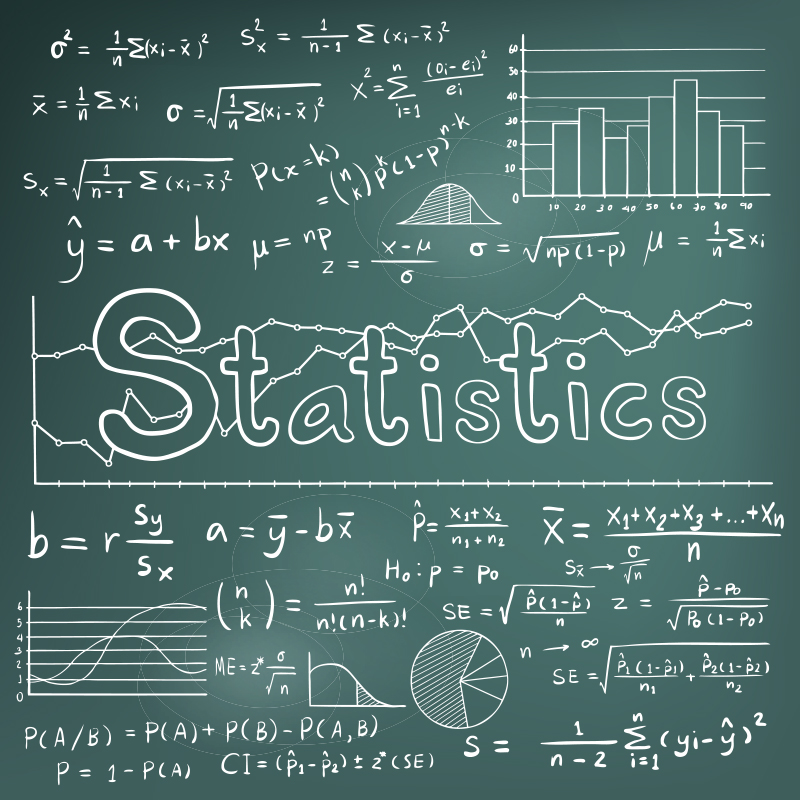
\includegraphics[width=1.0\paperwidth]{statistics-review.jpg}}
  \usebackgroundtemplate{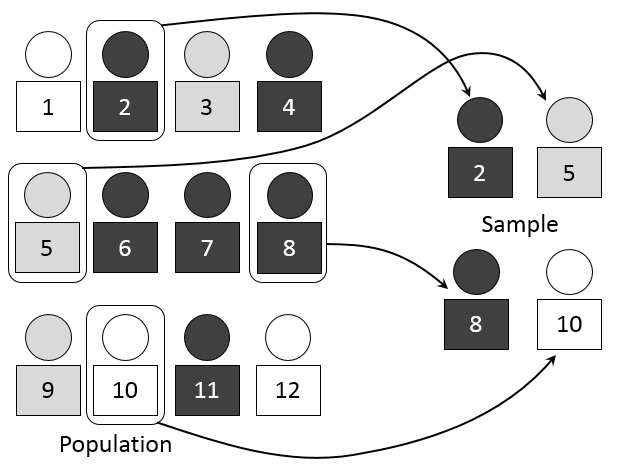
\includegraphics[scale=1.0]{Simple_random_sampling.png}}
  \begin{frame}[plain]
  
\begin{mdframed}[tikzsetting={draw=white,fill=white,fill opacity=0.6,draw opacity=0.4,
               line width=0pt},backgroundcolor=none,leftmargin=20,
               rightmargin=20,innertopmargin=4pt]
\begin{center}
\Huge \textbf{Sampling}
\end{center}
\end{mdframed}

  \end{frame}
}

%most reliant on human cognition
%limited only by cognition
%hypothesis generating scheme often functioning as a gateway into more statistical analysis

%%@@@@@@@@@@@@@@@@@@@@@@@@@@@@@@@@@@@@@@@@@@@@@@@@@
%\begin{frame}
%\frametitle{Napoleon's Progress}
%\begin{center}
%
\includegraphics[scale=0.4]{experiment.png}
%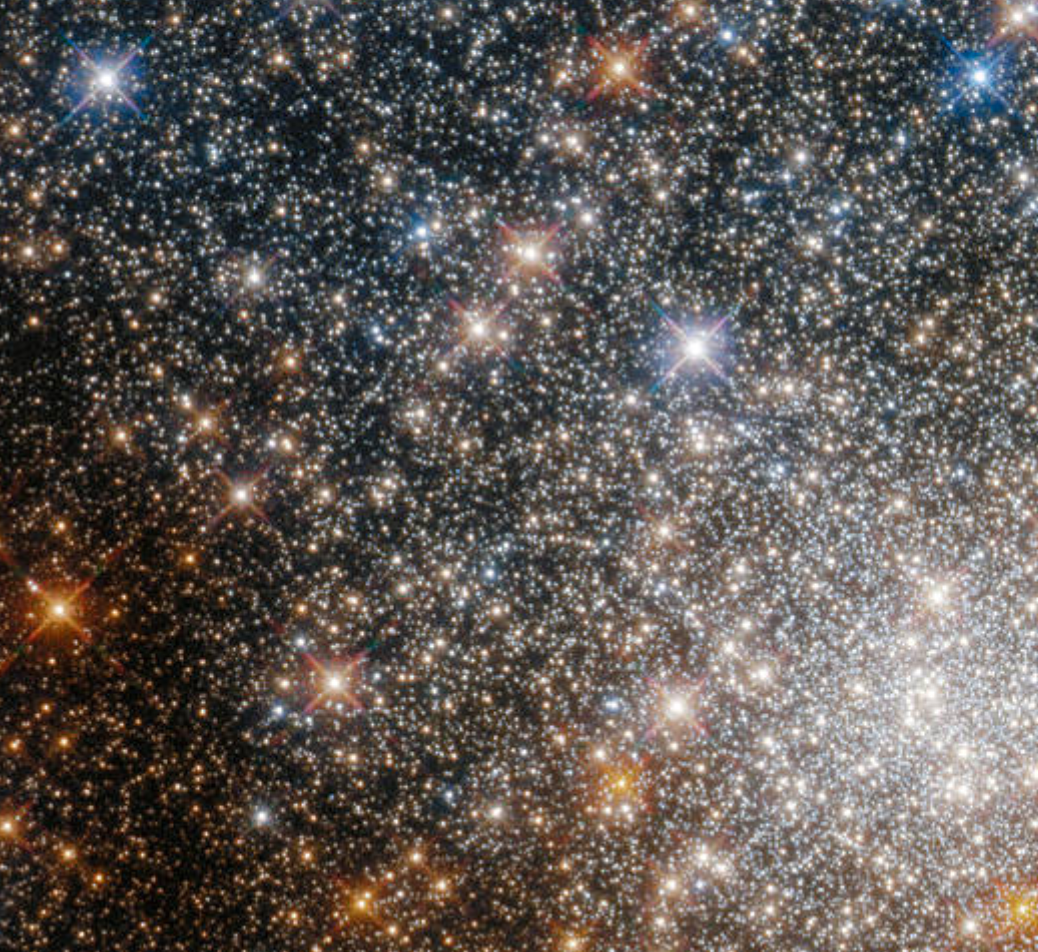
\includegraphics[scale=0.35]{stars.png}
%\end{center}
%
%\end{frame}

%@@@@@@@@@@@@@@@@@@@@@@@@@@@@@@@@@@@@@@@@@@@@@@@@@
\begin{frame}
\frametitle{Today:}

\begin{itemize}
\item What is sampling and what do we use it to do?
\bigskip
\bigskip
\bigskip
\item What is the effect of sampling variation/sample size on an estimate ?
\bigskip
\bigskip
\bigskip
\item What can go wrong with sampling and how can we fix it?

\end{itemize}

\end{frame}

%@@@@@@@@@@@@@@@@@@@@@@@@@@@@@@@@@@@@@@@@@@@@@@@@@
\begin{frame}
\frametitle{Definitions}
\begin{itemize}
\item \textbf{Population}: a `complete' group of $N$ objects, items, entities, or events of interest -- e.g. all adults living in the US;
\bigskip
\item \textbf{Sample}: a selected subset of $n$ individuals from a population -- e.g. 5,000 US adults appearing in a poll;
\bigskip
\item \textbf{Summary Statistic}: a summary of the information in a set of observations -- e.g. mean, median, mode, etc.;
\bigskip
\item[]\color{white} \textbf{Census}: a counting of all elements of the population;
\bigskip
\item[]\color{white} \textbf{Sampling}: the act of collecting a sample of size $n$ from a population of size $N$;
\begin{itemize} 
\item[]\color{white} sample only when we can’t perform a census;
\item[]\color{white} typically the sample size $n<<N$;
\end{itemize}
\bigskip
\item[]\color{white} \textbf{Sample Statistic}: a summary statistic computed from a sample that estimates the unknown population parameter.
\end{itemize}
\end{frame}

%@@@@@@@@@@@@@@@@@@@@@@@@@@@@@@@@@@@@@@@@@@@@@@@@@
\begin{frame}
\frametitle{Definitions}
\begin{itemize}
\item \textbf{Population}: a `complete' group of $N$ objects, items, entities, or events of interest -- e.g. all adults living in the US;
\bigskip
\item \textbf{Sample}: a selected subset of $n$ individuals from a population -- e.g. 5,000 US adults appearing in a poll;
\bigskip
\item \textbf{Summary Statistic}: a summary of the information in a set of observations -- e.g. mean, median, mode, etc.;
\bigskip
\item \textbf{Census}: a counting of all elements of the population;
\bigskip
\item[]\color{white} \textbf{Sampling}: the act of collecting a sample of size $n$ from a population of size $N$;
\begin{itemize} 
\item[]\color{white} sample only when we can’t perform a census;
\item[]\color{white} typically the sample size $n<<N$;
\end{itemize}
\bigskip
\item[]\color{white} \textbf{Sample Statistic}: a summary statistic computed from a sample that estimates the unknown population parameter.
\end{itemize}
\end{frame}

%@@@@@@@@@@@@@@@@@@@@@@@@@@@@@@@@@@@@@@@@@@@@@@@@@
\begin{frame}
\frametitle{Definitions}
\begin{itemize}
\item \textbf{Population}: a `complete' group of $N$ objects, items, entities, or events of interest -- e.g. all adults living in the US;
\bigskip
\item \textbf{Sample}: a selected subset of $n$ individuals from a population -- e.g. 5,000 US adults appearing in a poll;
\bigskip
\item \textbf{Summary Statistic}: a summary of the information in a set of observations -- e.g. mean, median, mode, etc.;
\bigskip
\item \textbf{Census}: a counting of all elements of the population;
\bigskip
\item \textbf{Sampling}: the act of collecting a sample of size $n$ from a population of size $N$;
\begin{itemize} 
\item sample only when we can’t perform a census;
\item typically the sample size $n<<N$;
\end{itemize}
\bigskip
\item \textbf{Sample Statistic}: a summary statistic computed from a sample that estimates the unknown population parameter.
\end{itemize}
\end{frame}

%@@@@@@@@@@@@@@@@@@@@@@@@@@@@@@@@@@@@@@@@@@@@@@@@@
\begin{frame}
\frametitle{A simple example -- marbles in a bag}

\begin{itemize}
\item Consider a bag full of marbles;
\begin{itemize}
\item the number of marbles in the bag is unknown;
\item there are multiple but unknown colors of marbles in the bag;
\item the fraction of any particular color of marbles in the bag is unknown;
\end{itemize}
\bigskip
\item Questions we could ask:
\begin{itemize}
\item How many marbles are in the bag?
\item How many colors of marbles are in the bag?
\item What is the fraction of blue marbles in the bag?
\end{itemize}
\bigskip
\item Assume we can't just dump the bag out or remove marbles from it permanently -- can we devise a process to answer any of these questions?
\bigskip
\item[]\color{white} What about the following:
\begin{enumerate}
\item[]\color{white} Stick a hand in the top of the bag and pull out handful of marbles;
\item[]\color{white} Observe them;
\item[]\color{white} Return them to the bag and then mix;
\item[]\color{white} Repeat.
\end{enumerate} 

\end{itemize}

\end{frame}

%@@@@@@@@@@@@@@@@@@@@@@@@@@@@@@@@@@@@@@@@@@@@@@@@@
\begin{frame}
\frametitle{A simple example -- marbles in a bag}

\begin{itemize}
\item Consider a bag full of marbles;
\begin{itemize}
\item the number of marbles in the bag is unknown;
\item there are multiple but unknown colors of marbles in the bag;
\item the fraction of any particular color of marbles in the bag is unknown;
\end{itemize}
\bigskip
\item Questions we could ask:
\begin{itemize}
\item How many marbles are in the bag?
\item How many colors of marbles are in the bag?
\item \textbf{What is the fraction of blue marbles in the bag?}
\end{itemize}
\bigskip
\item Assume we can't just dump the bag out or remove marbles from it permanently -- can we devise a process to answer any of these questions?
\bigskip
\item[]\color{white} What about the following:
\begin{enumerate}
\item[]\color{white} Stick a hand in the top of the bag and pull out handful of marbles;
\item[]\color{white} Observe them;
\item[]\color{white} Return them to the bag and then mix;
\item[]\color{white} Repeat.
\end{enumerate} 
\end{itemize}

\end{frame}

%@@@@@@@@@@@@@@@@@@@@@@@@@@@@@@@@@@@@@@@@@@@@@@@@@
\begin{frame}
\frametitle{A simple example -- marbles in a bag}

\begin{itemize}
\item Consider a bag full of marbles;
\begin{itemize}
\item the number of marbles in the bag is unknown;
\item there are multiple but unknown colors of marbles in the bag;
\item the fraction of any particular color of marbles in the bag is unknown;
\end{itemize}
\bigskip
\item Questions we could ask:
\begin{itemize}
\item How many marbles are in the bag?
\item How many colors of marbles are in the bag?
\item \textbf{What is the fraction of blue marbles in the bag?}
\end{itemize}
\bigskip
\item Assume we can't just dump the bag out or remove marbles from it permanently -- can we devise a process to answer any of these questions?
\bigskip
\item What about the following:
\begin{enumerate}
\item Stick a hand in the top of the bag and pull out handful of marbles;
\item Observe them;
\item Return them to the bag and then mix;
\item Repeat.
\end{enumerate} 
\end{itemize}

\end{frame}

%@@@@@@@@@@@@@@@@@@@@@@@@@@@@@@@@@@@@@@@@@@@@@@@@@
\begin{frame}
\begin{center}
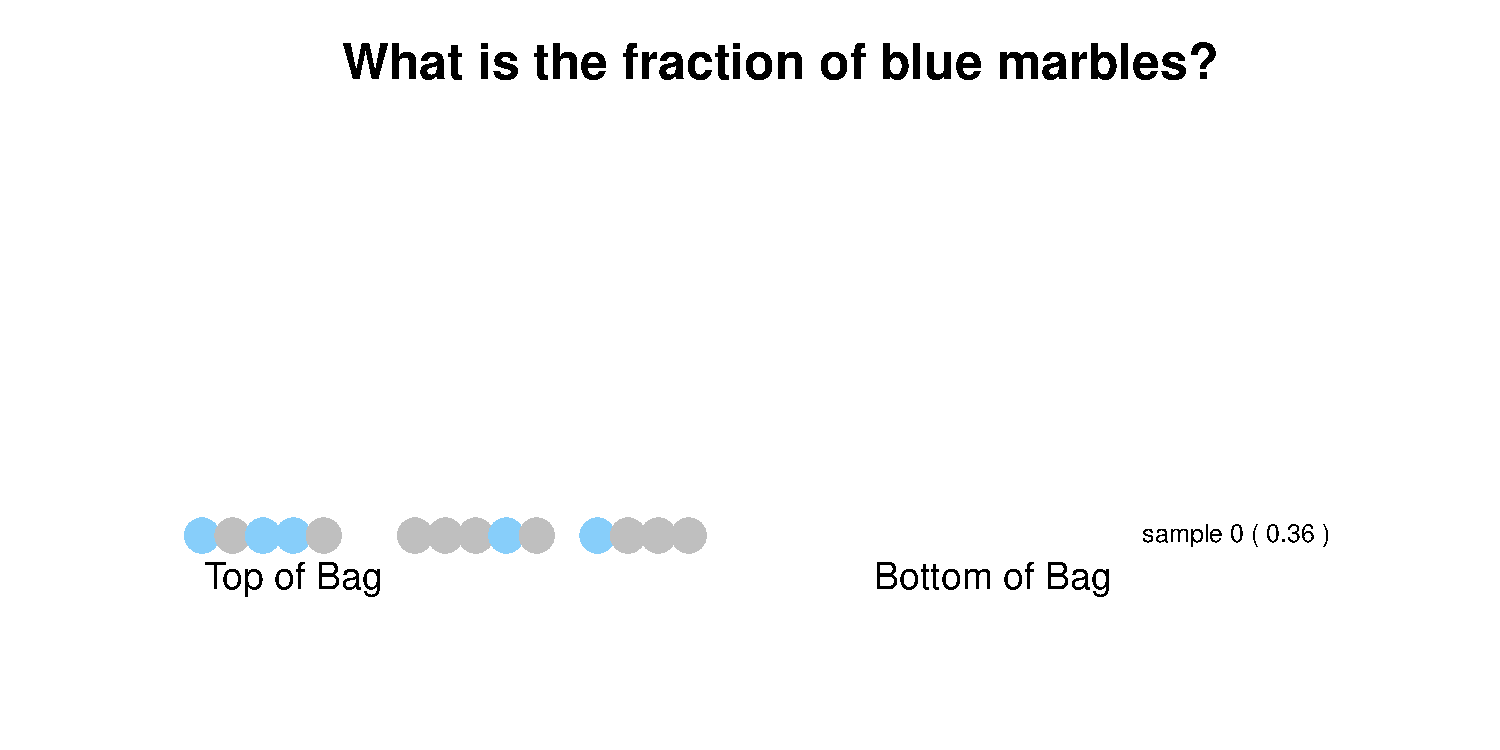
\includegraphics[scale=0.57]{sample_0.pdf}
\end{center}
\end{frame}

%@@@@@@@@@@@@@@@@@@@@@@@@@@@@@@@@@@@@@@@@@@@@@@@@@
\begin{frame}
\begin{center}
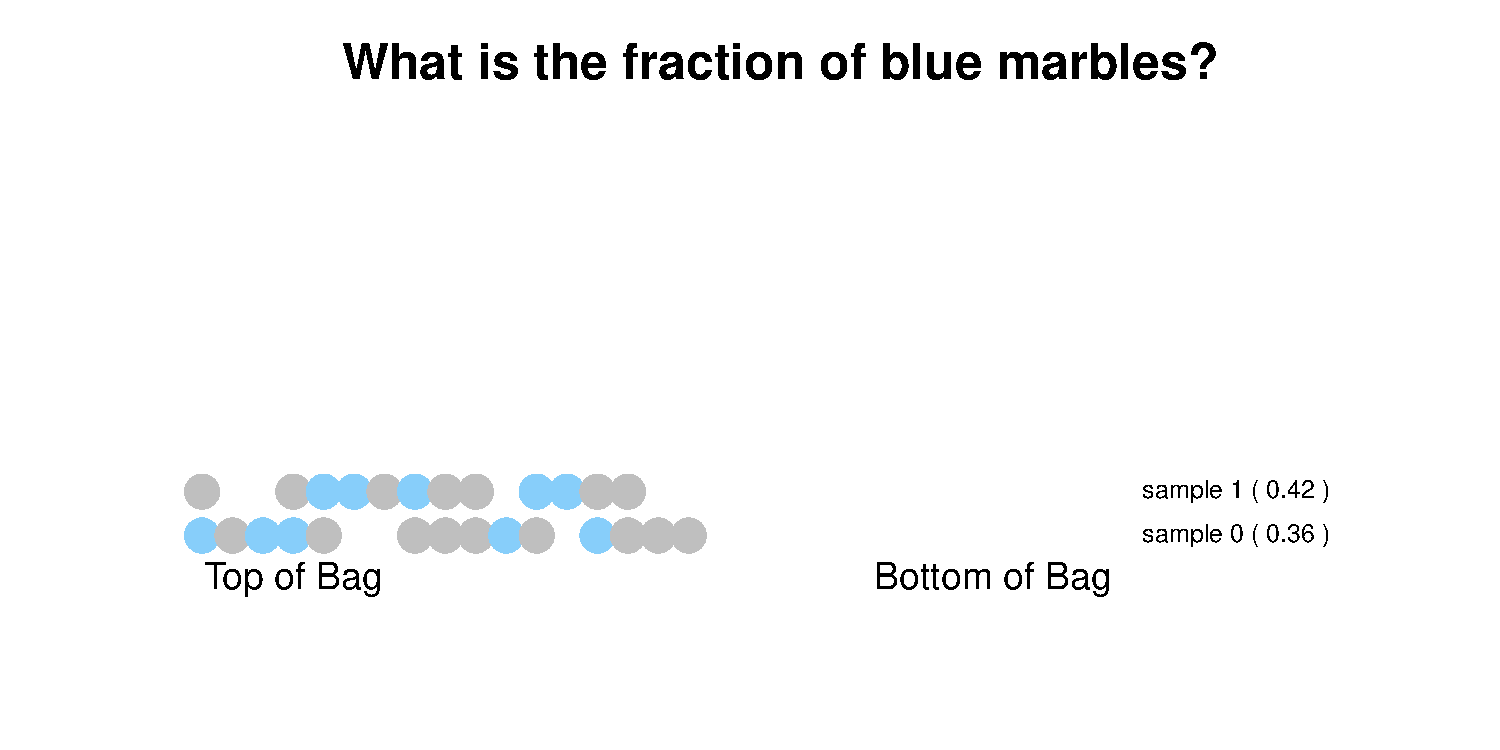
\includegraphics[scale=0.57]{sample_1.pdf}
\end{center}
\end{frame}

%@@@@@@@@@@@@@@@@@@@@@@@@@@@@@@@@@@@@@@@@@@@@@@@@@
\begin{frame}
\begin{center}
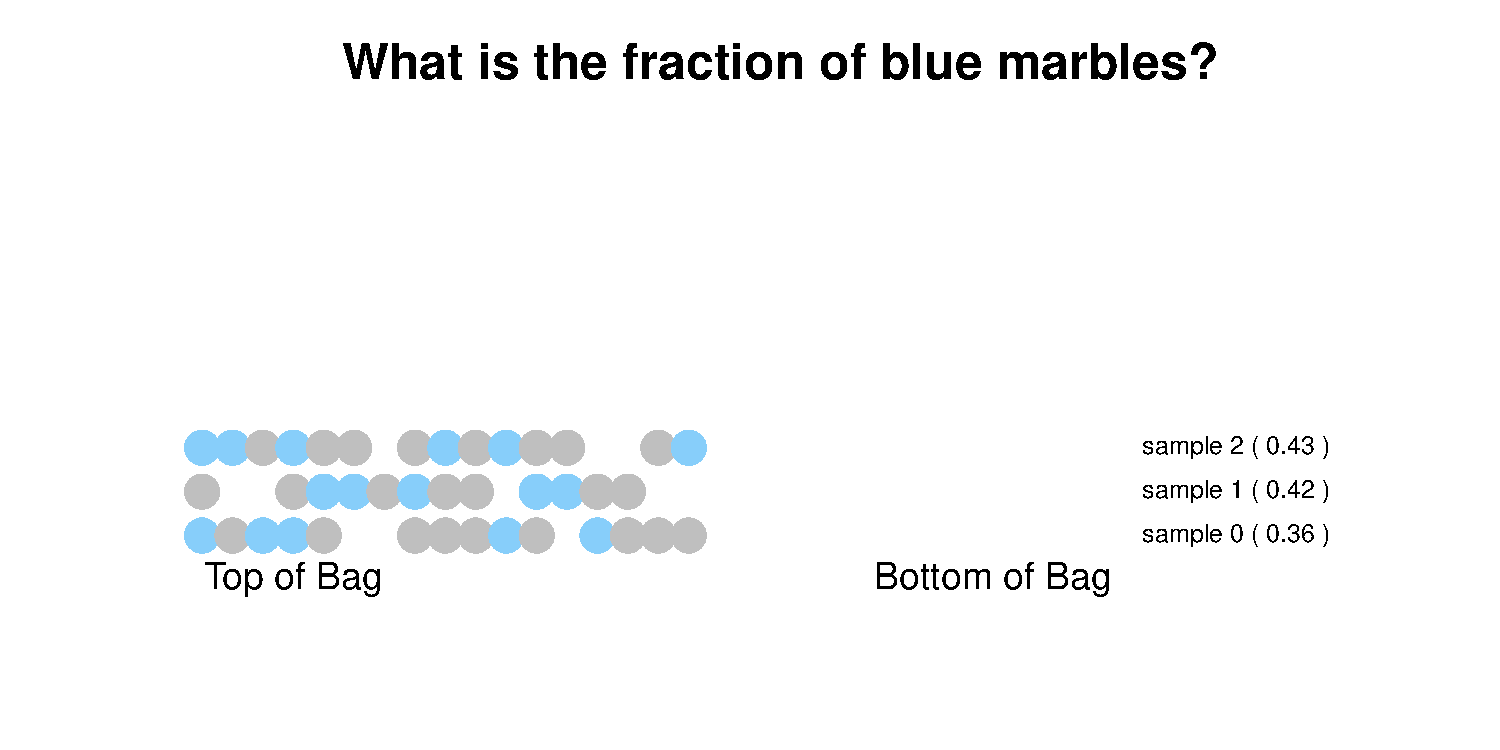
\includegraphics[scale=0.57]{sample_2.pdf}
\end{center}
\end{frame}

%@@@@@@@@@@@@@@@@@@@@@@@@@@@@@@@@@@@@@@@@@@@@@@@@@
\begin{frame}
\begin{center}
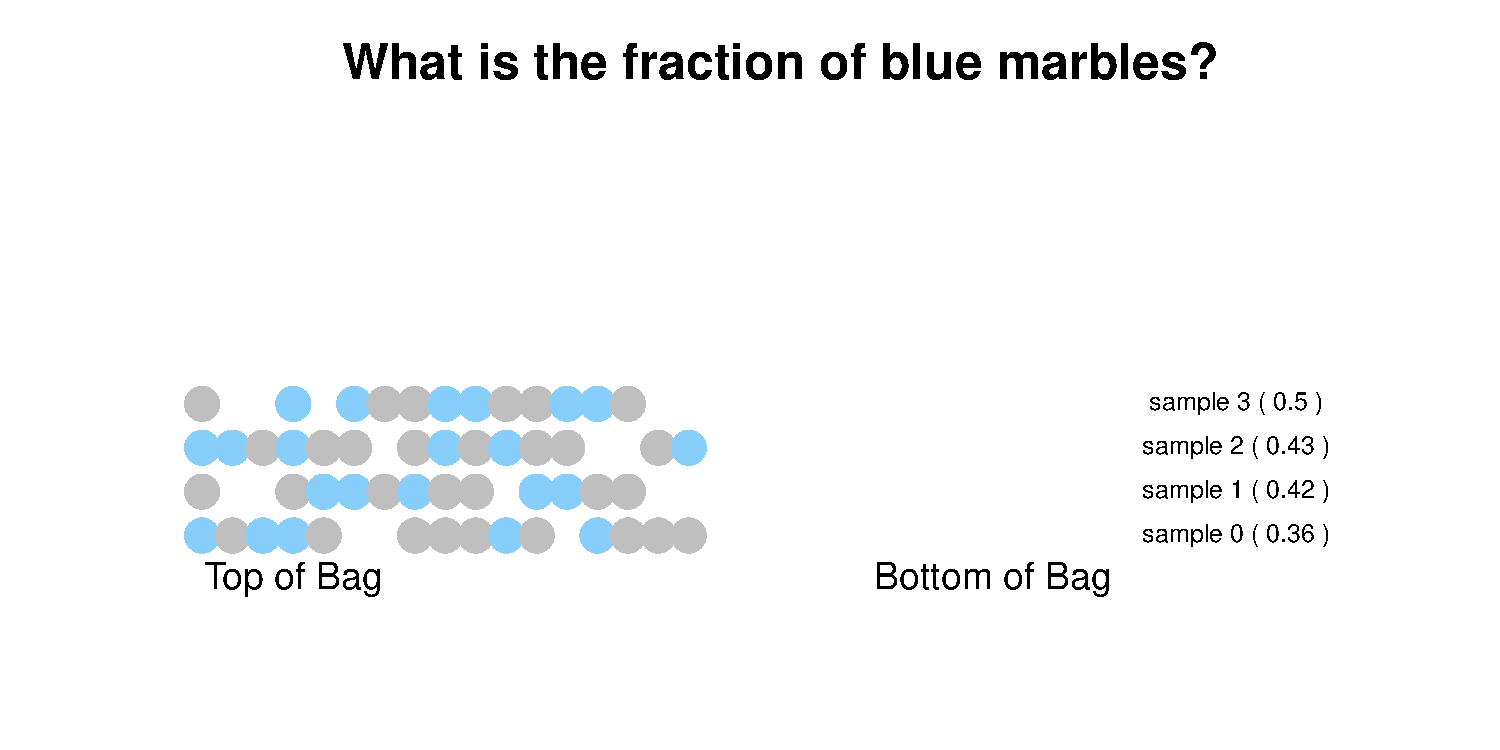
\includegraphics[scale=0.57]{sample_3.pdf}
\end{center}
\end{frame}

%@@@@@@@@@@@@@@@@@@@@@@@@@@@@@@@@@@@@@@@@@@@@@@@@@
\begin{frame}
\begin{center}
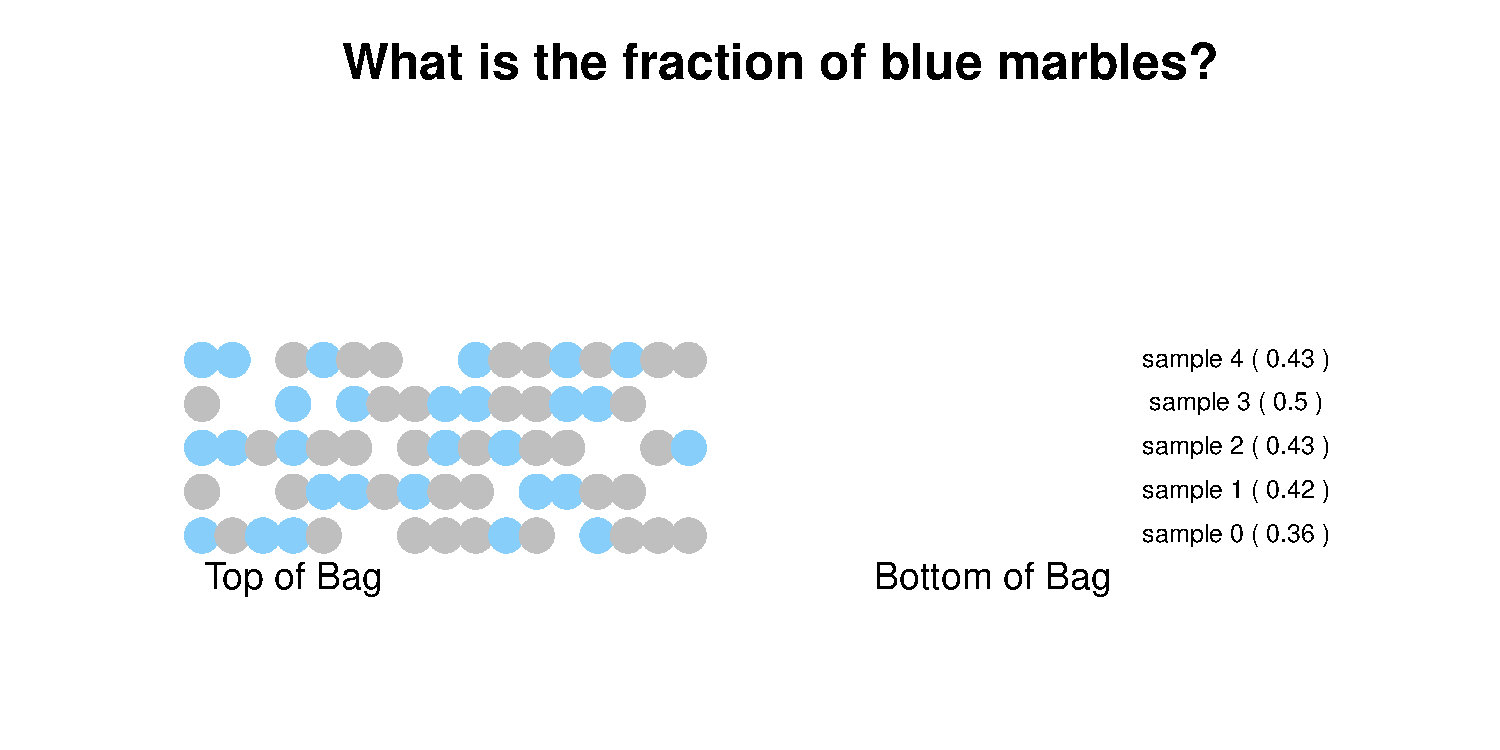
\includegraphics[scale=0.57]{sample_4.pdf}
\end{center}
\end{frame}

%@@@@@@@@@@@@@@@@@@@@@@@@@@@@@@@@@@@@@@@@@@@@@@@@@
\begin{frame}
\begin{center}
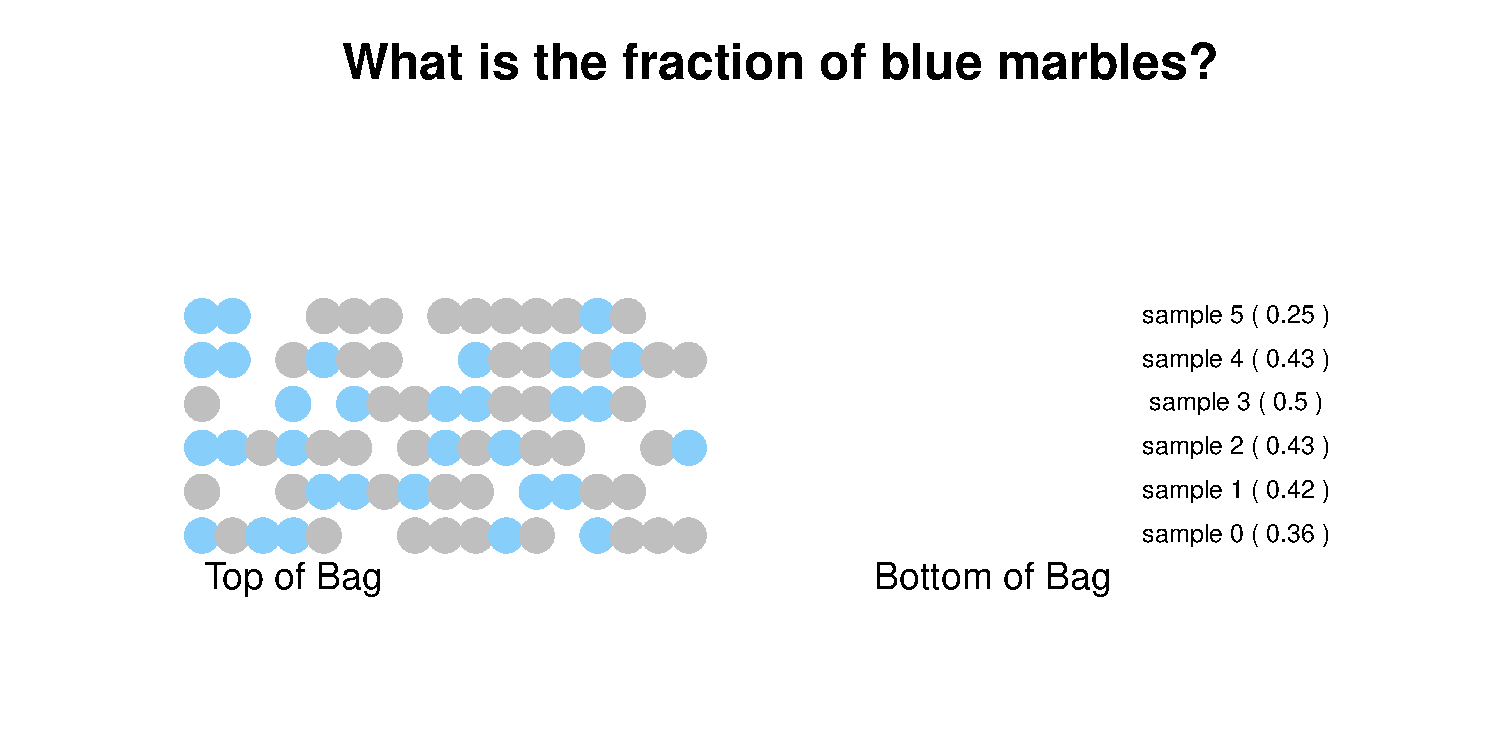
\includegraphics[scale=0.57]{sample_5.pdf}
\end{center}
\end{frame}

%@@@@@@@@@@@@@@@@@@@@@@@@@@@@@@@@@@@@@@@@@@@@@@@@@
\begin{frame}
\begin{center}
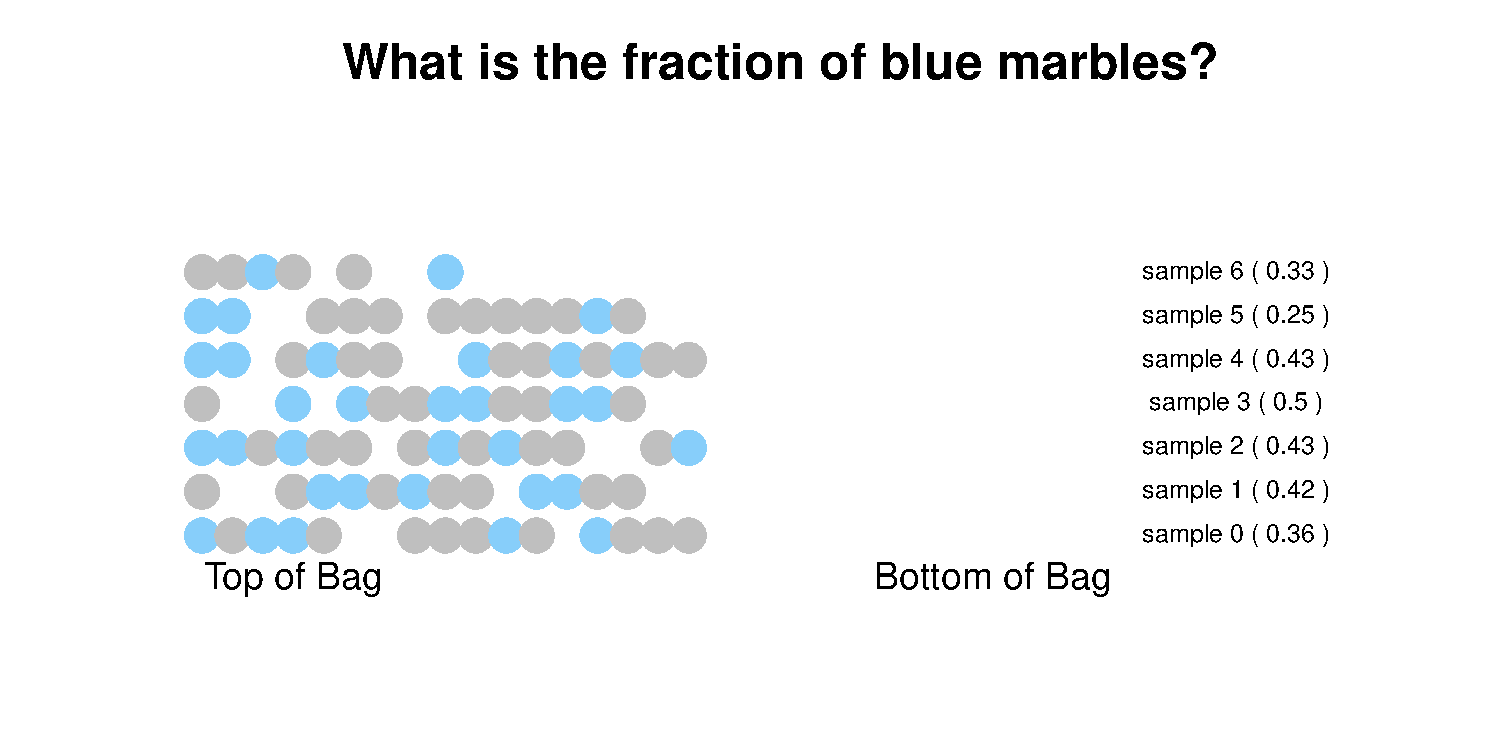
\includegraphics[scale=0.57]{sample_6.pdf}
\end{center}
\end{frame}

%@@@@@@@@@@@@@@@@@@@@@@@@@@@@@@@@@@@@@@@@@@@@@@@@@
\begin{frame}
\begin{center}
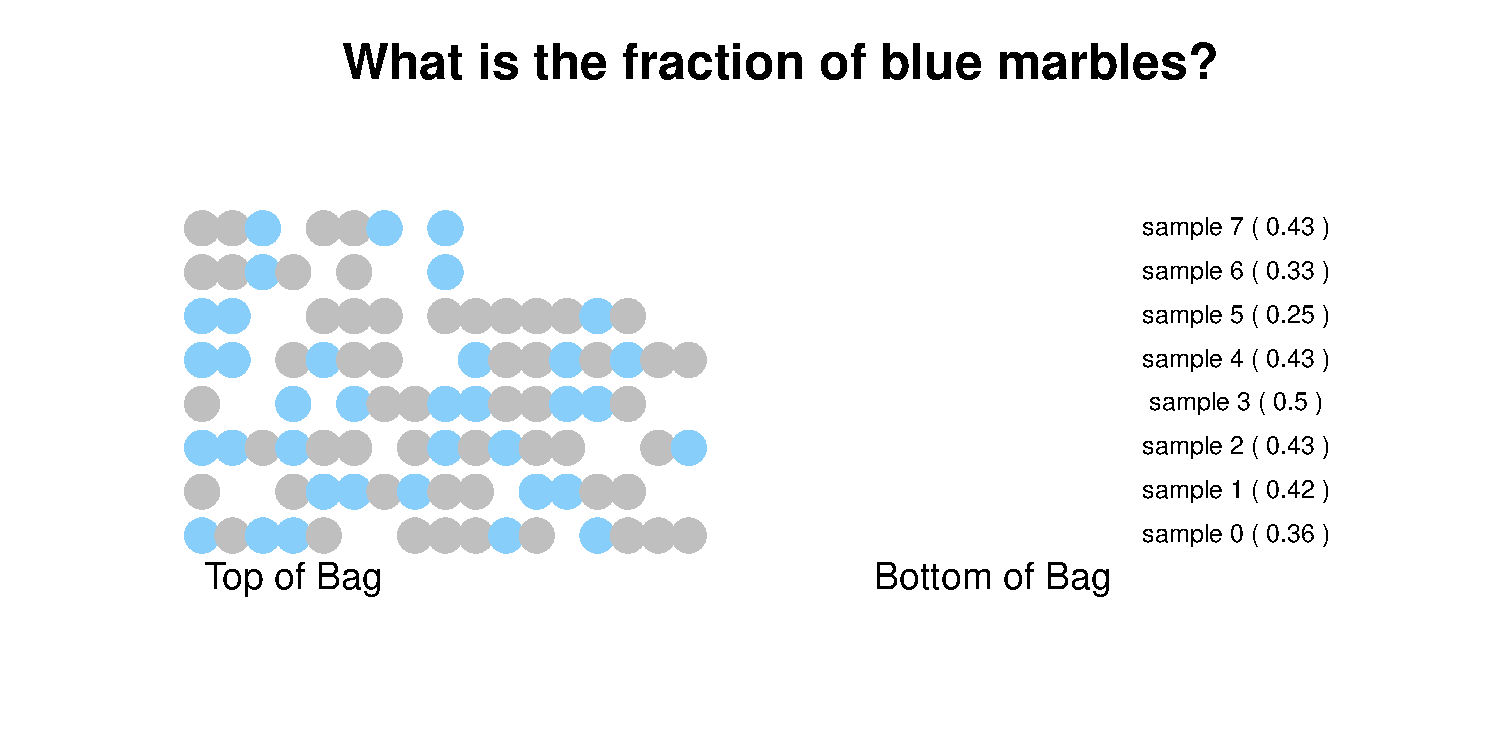
\includegraphics[scale=0.57]{sample_7.pdf}
\end{center}
\end{frame}

%@@@@@@@@@@@@@@@@@@@@@@@@@@@@@@@@@@@@@@@@@@@@@@@@@
\begin{frame}
\begin{center}
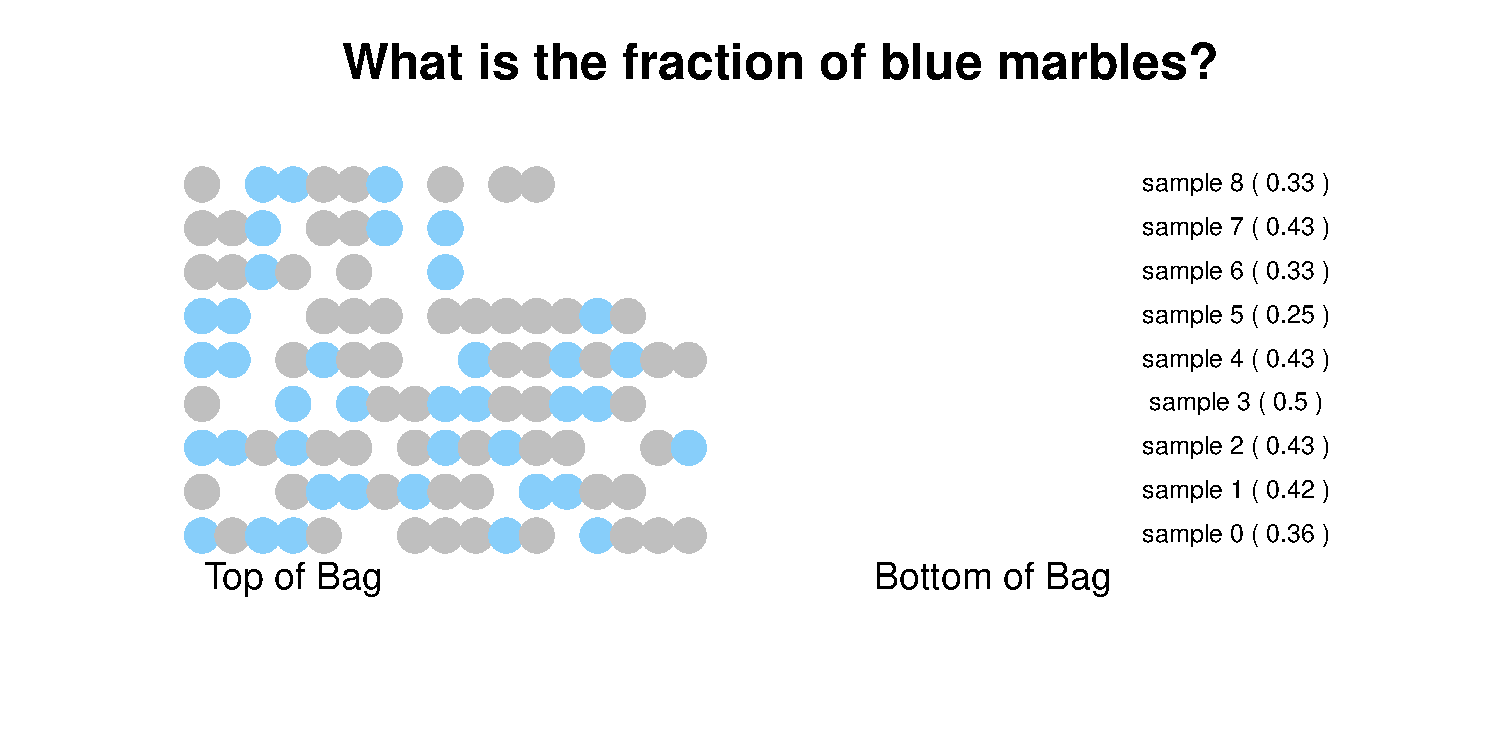
\includegraphics[scale=0.57]{sample_8.pdf}
\end{center}
\end{frame}

%@@@@@@@@@@@@@@@@@@@@@@@@@@@@@@@@@@@@@@@@@@@@@@@@@
\begin{frame}
\begin{center}
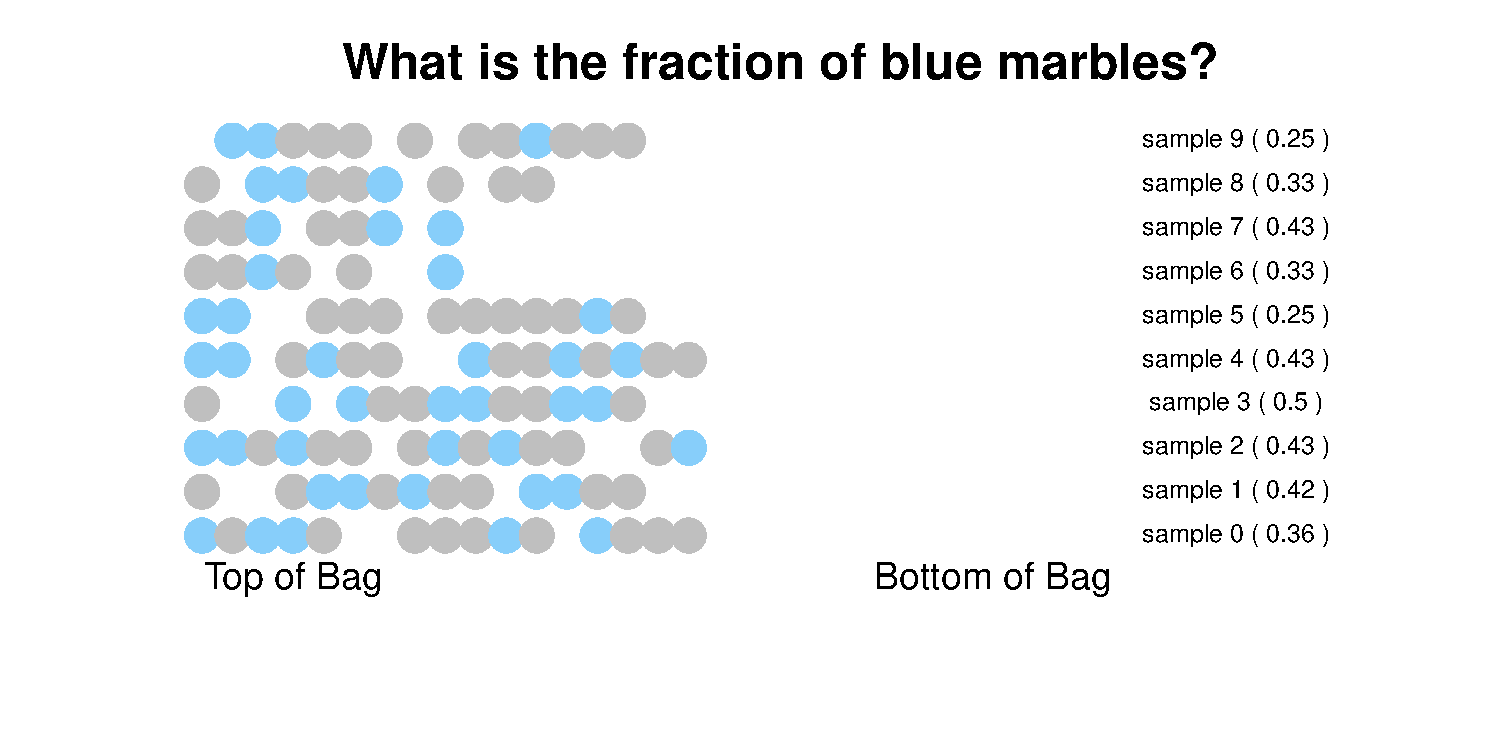
\includegraphics[scale=0.57]{sample_9.pdf}
\end{center}
\end{frame}

%@@@@@@@@@@@@@@@@@@@@@@@@@@@@@@@@@@@@@@@@@@@@@@@@@
\begin{frame}
\begin{center}
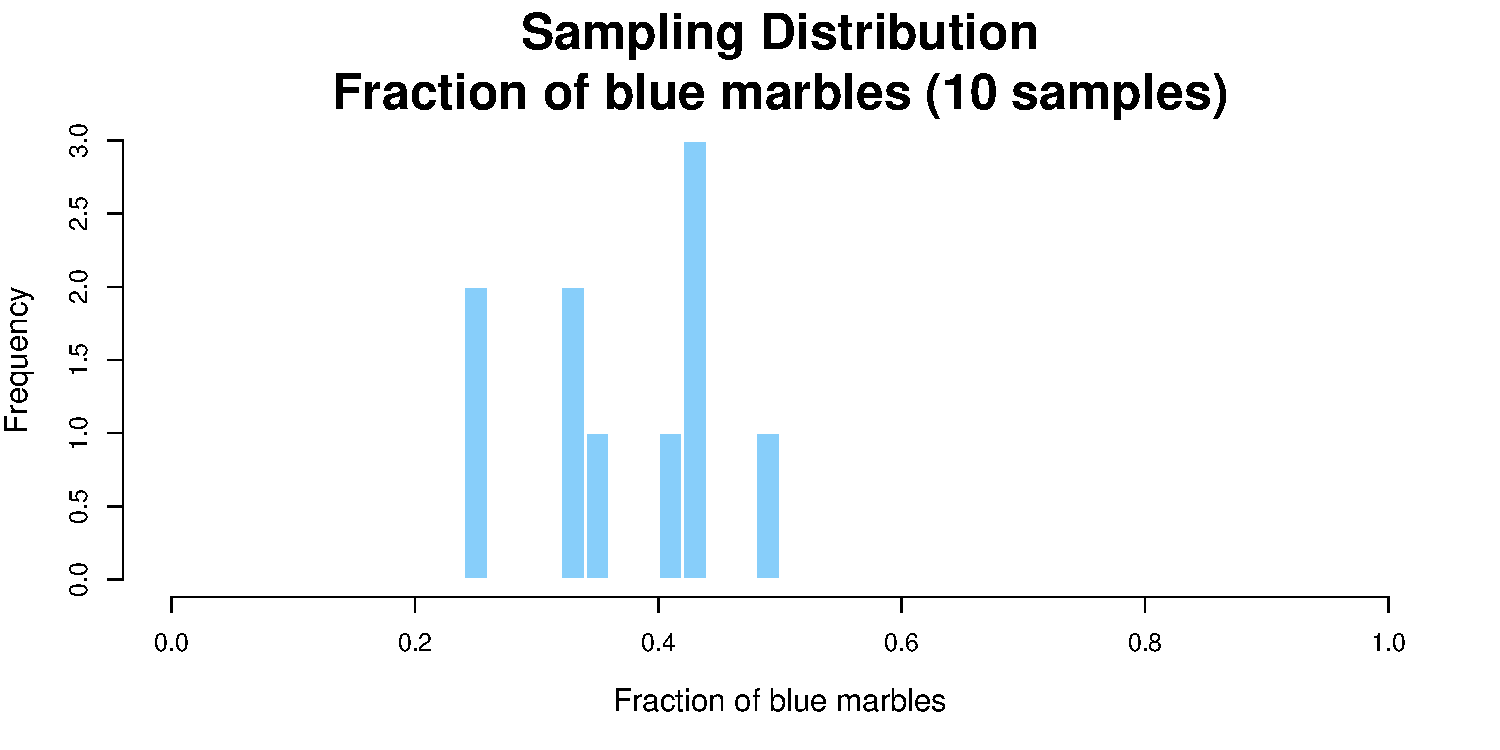
\includegraphics[scale=0.57]{hist_10_samples.pdf}
\end{center}
\end{frame}

%@@@@@@@@@@@@@@@@@@@@@@@@@@@@@@@@@@@@@@@@@@@@@@@@@
\begin{frame}
\begin{center}
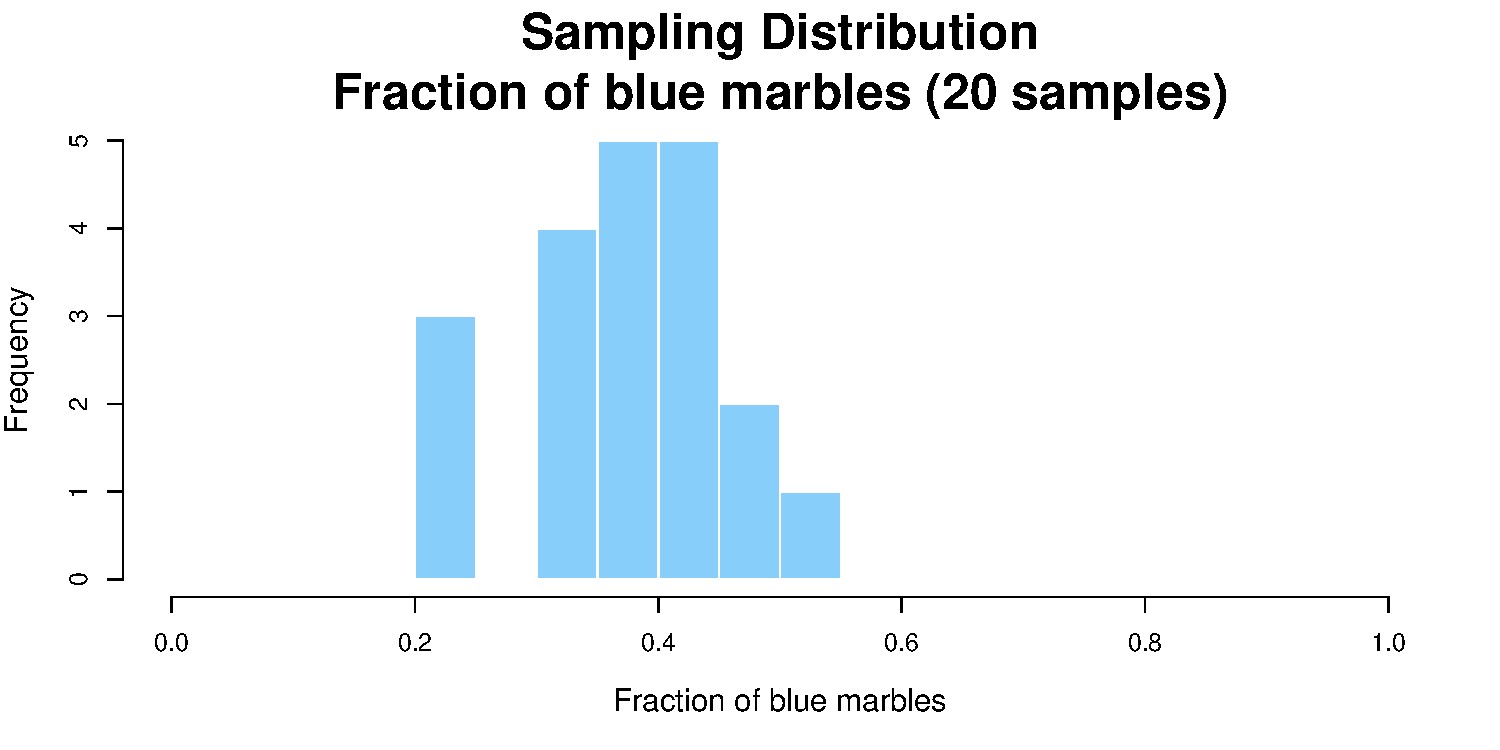
\includegraphics[scale=0.57]{hist_20_samples.pdf}
\end{center}
\end{frame}

%@@@@@@@@@@@@@@@@@@@@@@@@@@@@@@@@@@@@@@@@@@@@@@@@@
\begin{frame}
\begin{center}
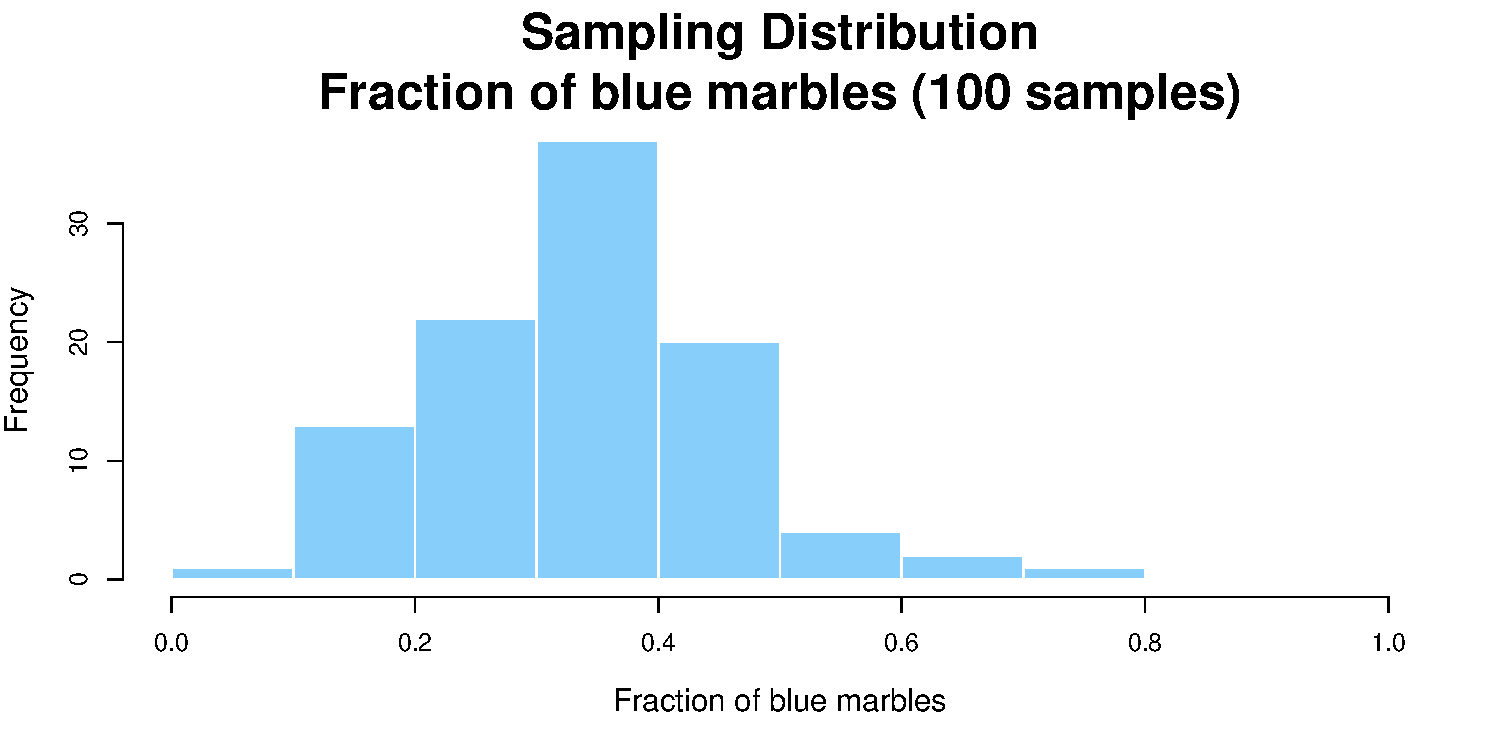
\includegraphics[scale=0.57]{hist_100_samples.pdf}
\end{center}
\end{frame}

%@@@@@@@@@@@@@@@@@@@@@@@@@@@@@@@@@@@@@@@@@@@@@@@@@
\begin{frame}
\begin{center}
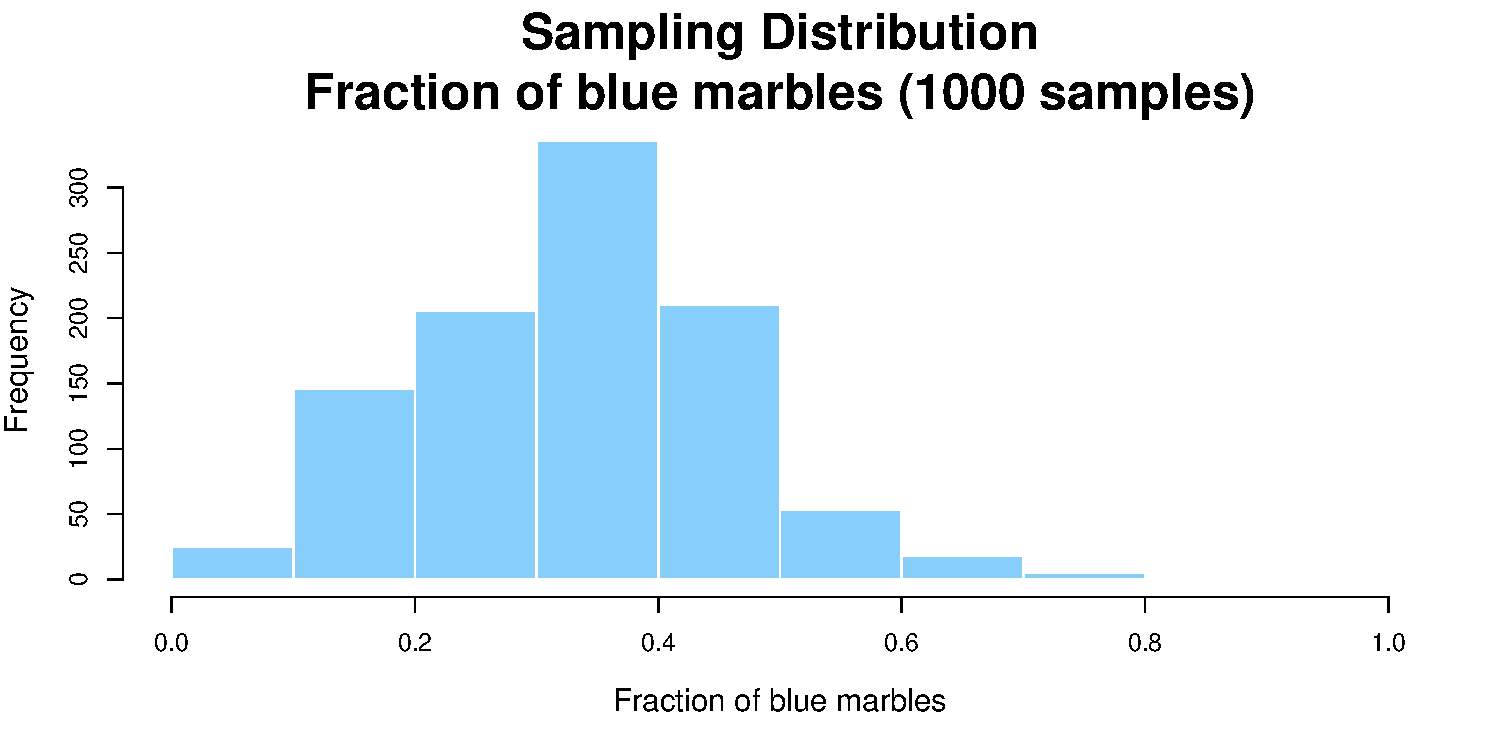
\includegraphics[scale=0.57]{hist_1000_samples.pdf}
\end{center}
\end{frame}

%@@@@@@@@@@@@@@@@@@@@@@@@@@@@@@@@@@@@@@@@@@@@@@@@@
\begin{frame}
\begin{center}
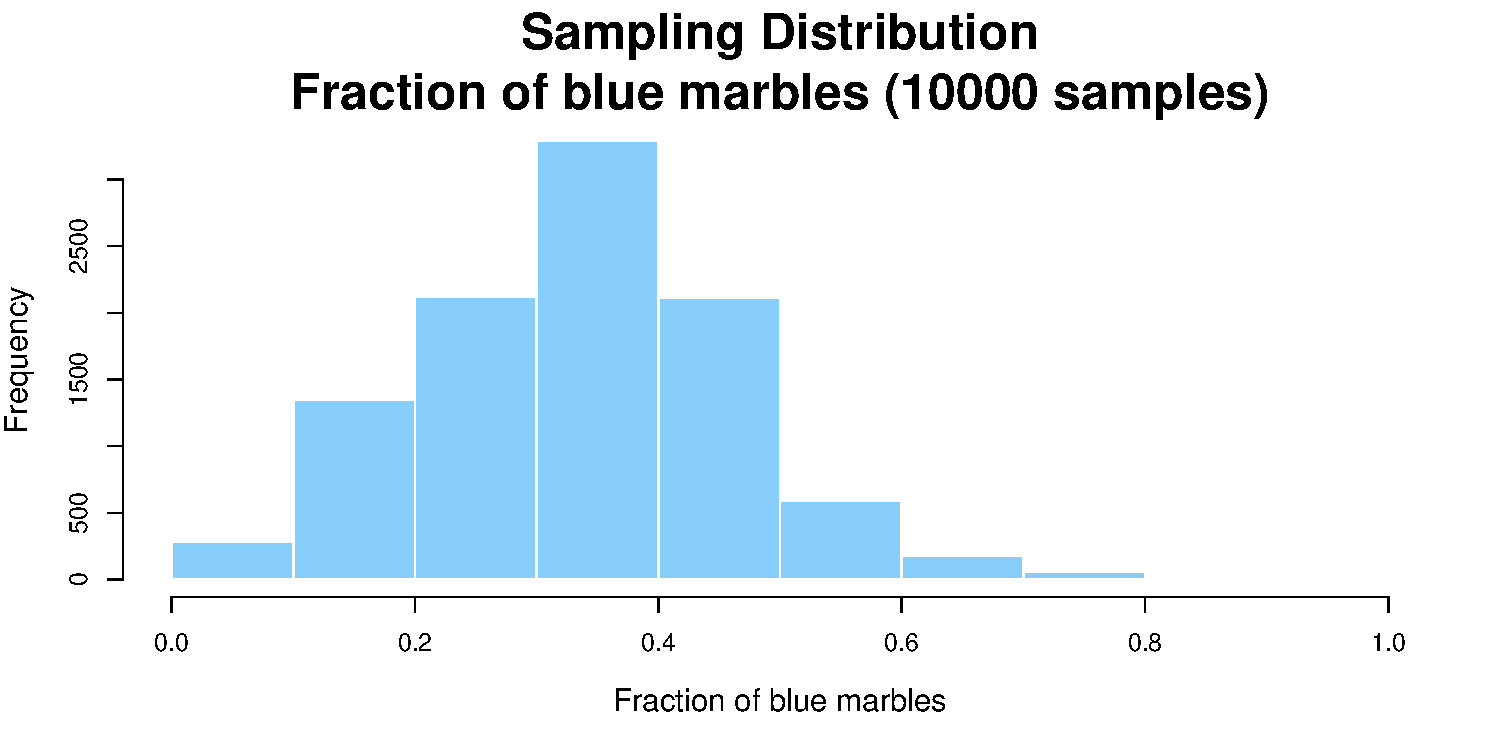
\includegraphics[scale=0.57]{hist_10000_samples.pdf}
\end{center}
\end{frame}

%@@@@@@@@@@@@@@@@@@@@@@@@@@@@@@@@@@@@@@@@@@@@@@@@@
\begin{frame}
\frametitle{Summarizing what we've learned from doing this...}
\begin{itemize}
\item What should we conclude from our samples about the fraction of blue marbles in the bag?  Consider taking the average of the first 10:
\begin{align*}
\frac{0.36 + 0.42 + 0.43 + 0.5 + 0.43 + 0.25 + 0.33 + 0.43 + 0.33 + 0.25}{10} = 0.373;
\end{align*}
\bigskip

\item What is a reasonable measurement of variation around this?
\begin{itemize}
\item[]\color{white} Option 1 -- look at it empirically:
\begin{align*}
\color{white}0.25,\underbrace{\textbf{0.25},0.33,0.33,0.36,0.42,0.43,0.43,\textbf{0.43}}_{\mbox{middle 80\% of data}},0.5
\end{align*}
\item[]\color{white} Option 2 -- compute the sample standard deviation:
\begin{align*}
\color{white}\sigma = \sqrt{\frac{1}{n-1}\sum_{i=1}^n(x_i - \overline{x})^2} = \sqrt{\frac{(0.25 - 0.373)^2 + \hdots + (0.5 - 0.373)^2}{10 - 1}}\approx 0.083.
\end{align*}
\end{itemize}

\end{itemize}
\end{frame}

%@@@@@@@@@@@@@@@@@@@@@@@@@@@@@@@@@@@@@@@@@@@@@@@@@
\begin{frame}
\frametitle{Summarizing what we've learned from doing this...}
\begin{itemize}
\item What should we conclude from our samples about the fraction of blue marbles in the bag?  Consider taking the average of the first 10:
\begin{align*}
\frac{0.36 + 0.42 + 0.43 + 0.5 + 0.43 + 0.25 + 0.33 + 0.43 + 0.33 + 0.25}{10} = 0.373;
\end{align*}
\bigskip

\item What is a reasonable measurement of variation around this?
\begin{itemize}
\item Option 1 -- look at it empirically:
\begin{align*}
0.25,\underbrace{\textbf{0.25},0.33,0.33,0.36,0.42,0.43,0.43,\textbf{0.43}}_{\mbox{middle 80\% of data}},0.5
\end{align*}
\item Option 2 -- compute the sample standard deviation:
\begin{align*}
\sigma = \sqrt{\frac{1}{n-1}\sum_{i=1}^n(x_i - \overline{x})^2} = \sqrt{\frac{(0.25 - 0.373)^2 + \hdots + (0.5 - 0.373)^2}{10 - 1}}\approx 0.083.
\end{align*}
\end{itemize}

\end{itemize}
\end{frame}

%%@@@@@@@@@@@@@@@@@@@@@@@@@@@@@@@@@@@@@@@@@@@@@@@@@
%\begin{frame}
%\begin{center}
%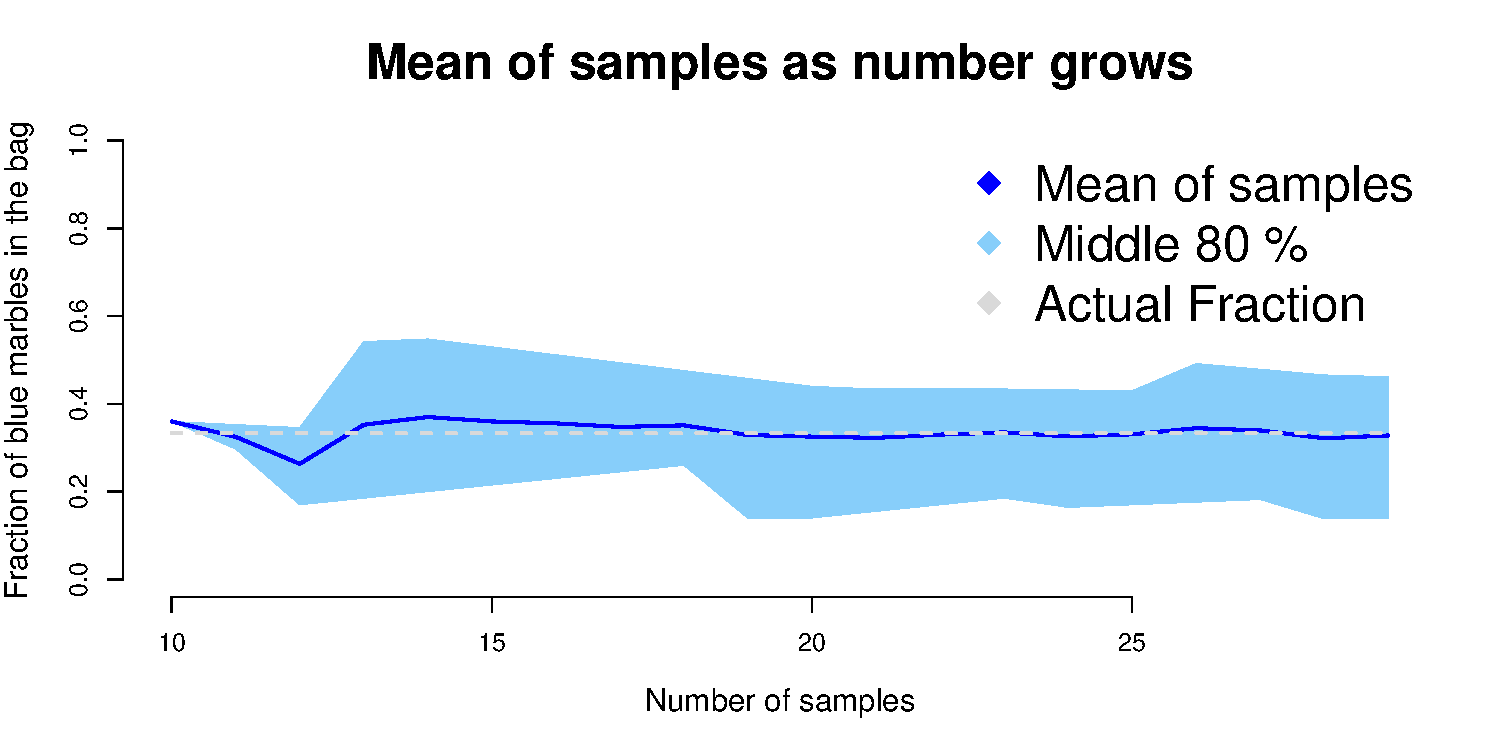
\includegraphics[scale=0.57]{means20_samples.pdf}
%\end{center}
%\end{frame}

%@@@@@@@@@@@@@@@@@@@@@@@@@@@@@@@@@@@@@@@@@@@@@@@@@
\begin{frame}
\begin{center}
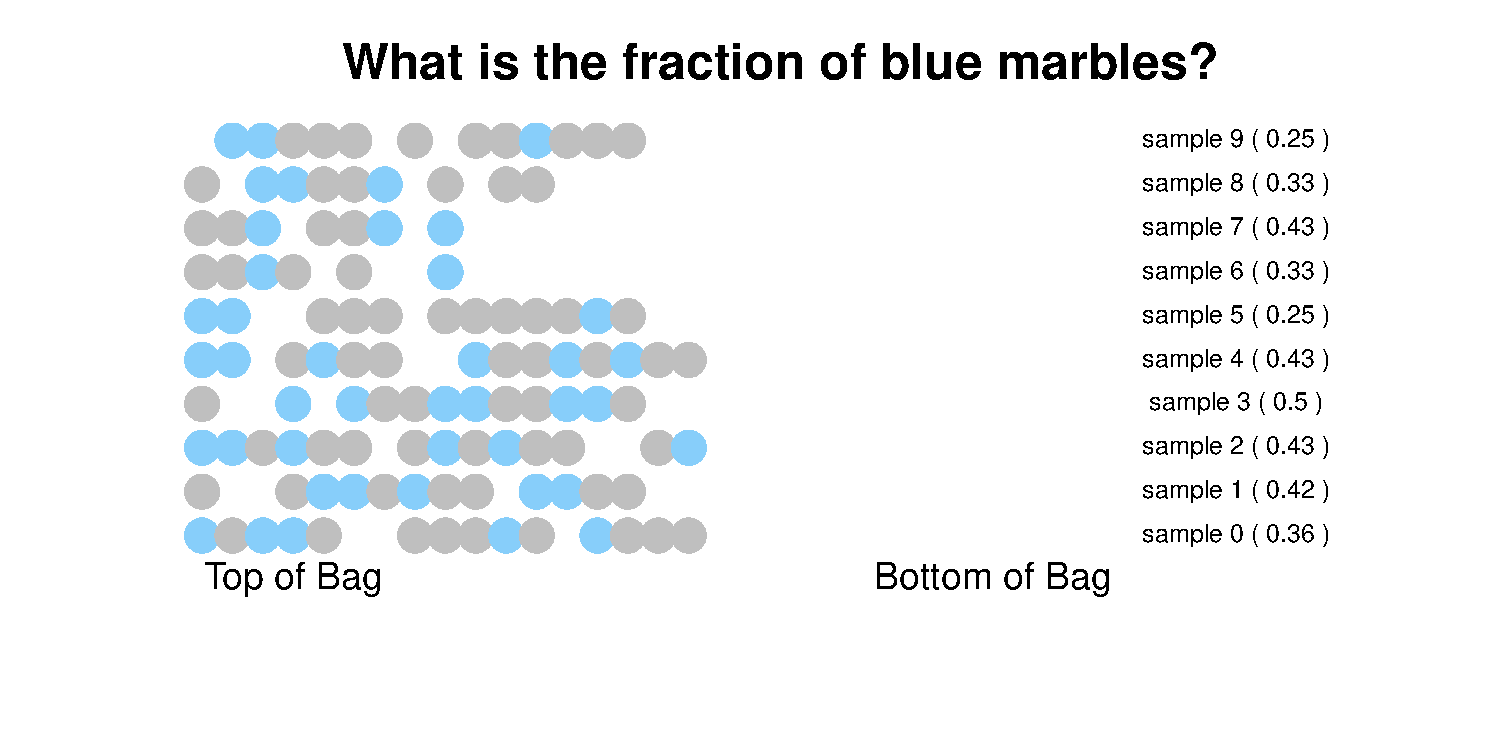
\includegraphics[scale=0.57]{sample_9.pdf}
\end{center}
\end{frame}

%@@@@@@@@@@@@@@@@@@@@@@@@@@@@@@@@@@@@@@@@@@@@@@@@@
\begin{frame}
\begin{center}
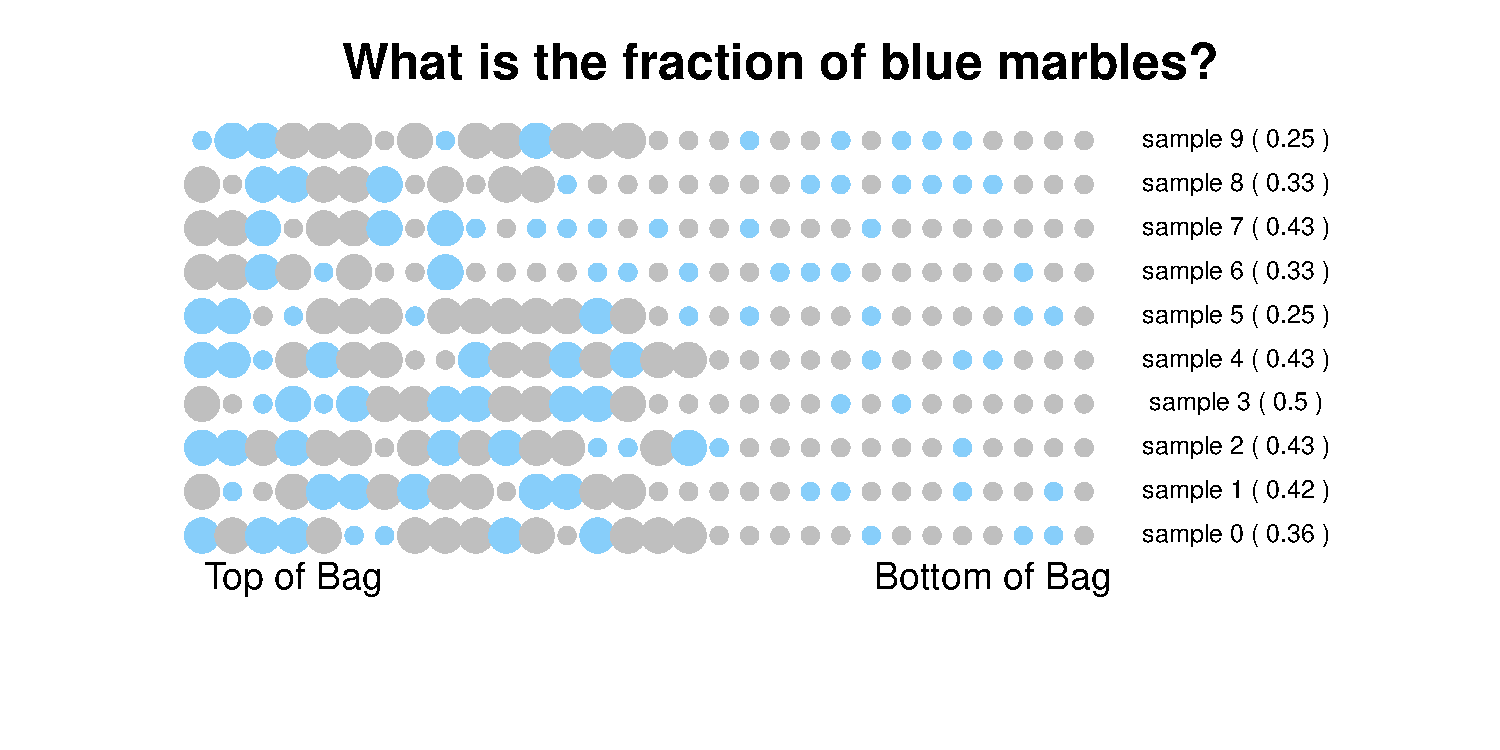
\includegraphics[scale=0.57]{sample_full.pdf}
\end{center}
\end{frame}

%@@@@@@@@@@@@@@@@@@@@@@@@@@@@@@@@@@@@@@@@@@@@@@@@@
\begin{frame}
\begin{center}
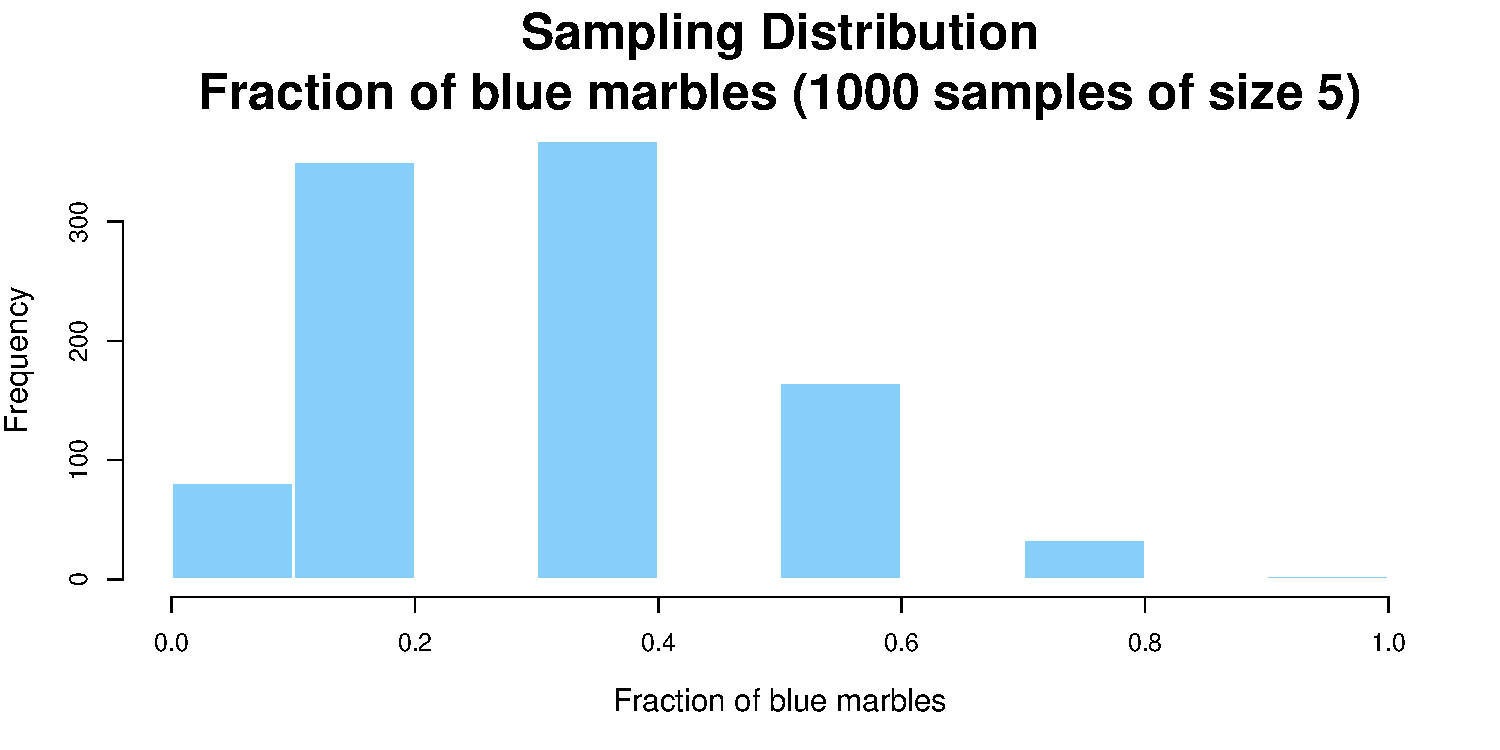
\includegraphics[scale=0.57]{hist_1000_samples_5_size.pdf}
\end{center}
\end{frame}

%@@@@@@@@@@@@@@@@@@@@@@@@@@@@@@@@@@@@@@@@@@@@@@@@@
\begin{frame}
\begin{center}
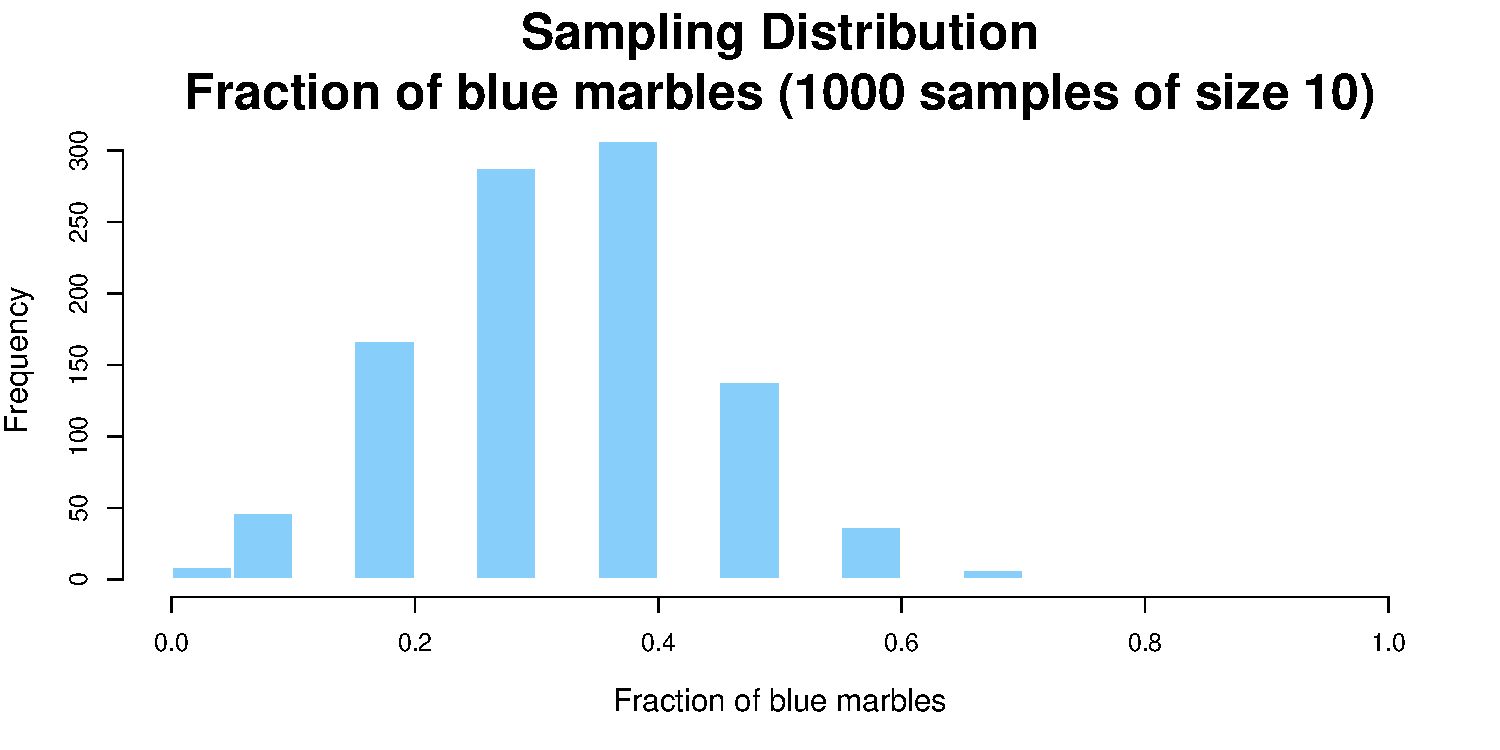
\includegraphics[scale=0.57]{hist_1000_samples_10_size.pdf}
\end{center}
\end{frame}

%@@@@@@@@@@@@@@@@@@@@@@@@@@@@@@@@@@@@@@@@@@@@@@@@@
\begin{frame}
\begin{center}
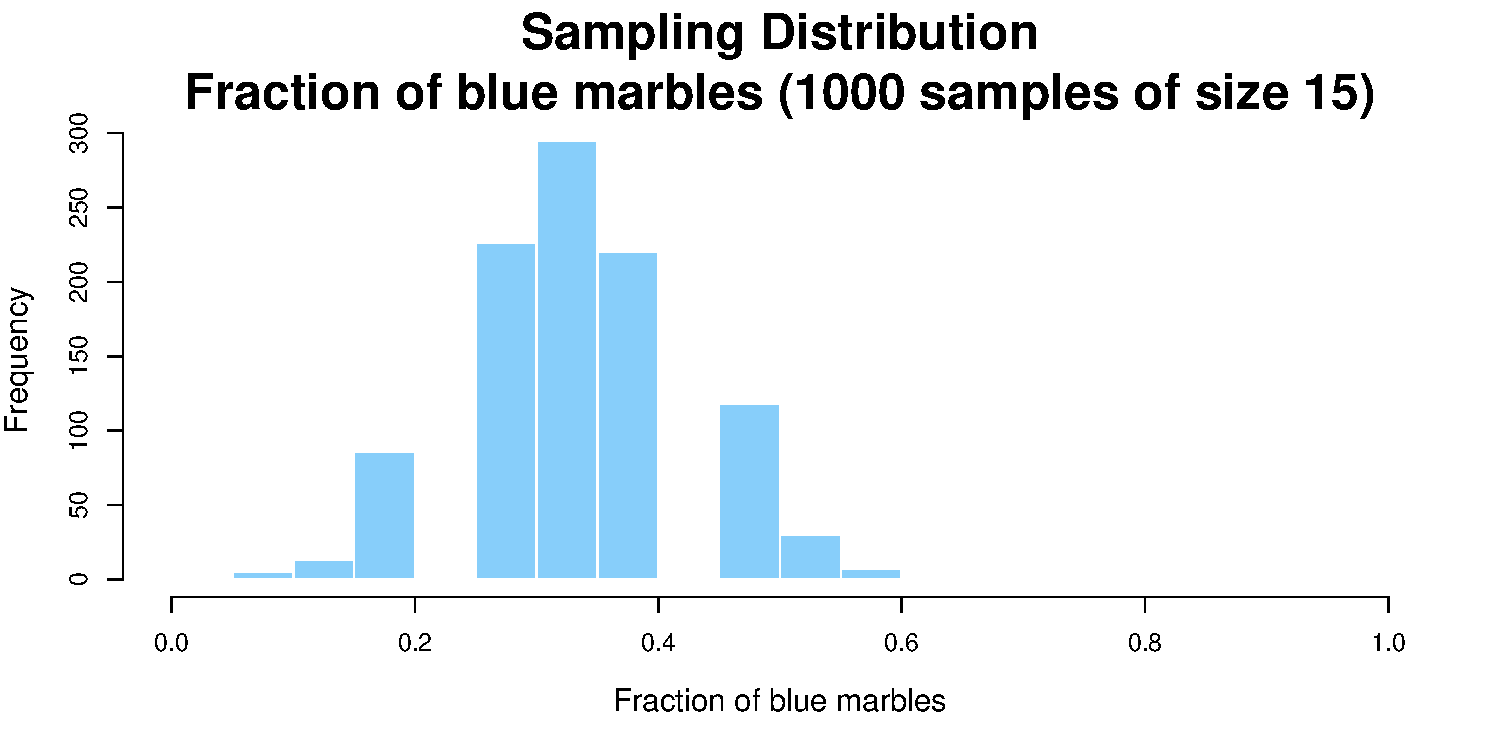
\includegraphics[scale=0.57]{hist_1000_samples_15_size.pdf}
\end{center}
\end{frame}

%@@@@@@@@@@@@@@@@@@@@@@@@@@@@@@@@@@@@@@@@@@@@@@@@@
\begin{frame}
\begin{center}
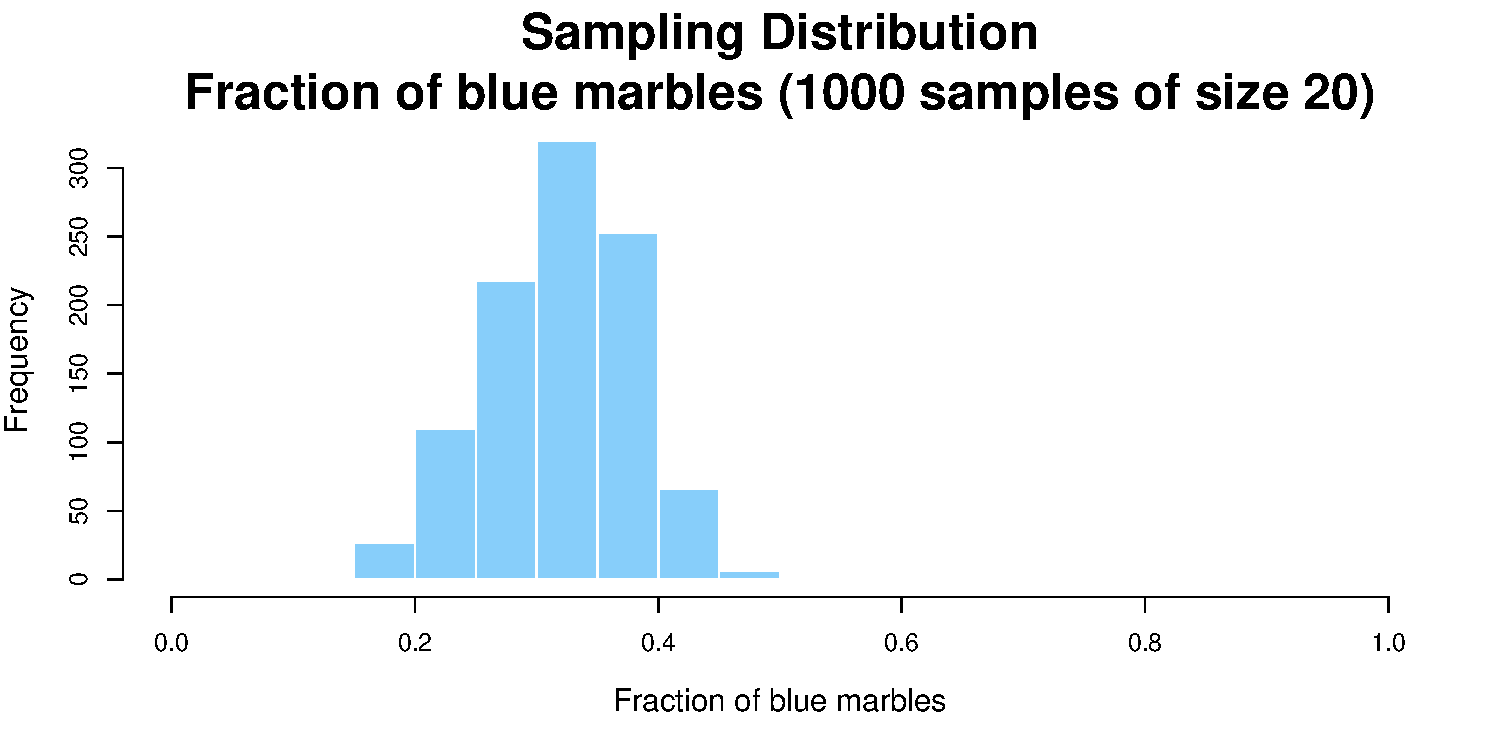
\includegraphics[scale=0.57]{hist_1000_samples_20_size.pdf}
\end{center}
\end{frame}

%@@@@@@@@@@@@@@@@@@@@@@@@@@@@@@@@@@@@@@@@@@@@@@@@@
\begin{frame}
\frametitle{A simple example -- marbles in a bag (take 2)}

\begin{itemize}
\item Consider a bag full of marbles;
\begin{itemize}
\item the number of marbles in the bag is unknown;
\item there are multiple but unknown colors of marbles in the bag;
\item the fraction of any particular color of marbles in the bag is unknown;
\end{itemize}
\bigskip
\item Questions we could ask:
\begin{itemize}
\item How many marbles are in the bag?
\item How many colors of marbles are in the bag?
\item \textbf{What is the fraction of blue marbles in the bag?}
\end{itemize}
\bigskip
\item Assume we can't just dump the bag out or remove marbles from it permanently -- can we devise a process to answer any of these questions?
\bigskip
\item What about the following:
\begin{enumerate}
\item Stick a hand in the top of the bag and pull out handful of marbles;
\item Observe them;
\item Return them to the bag and then mix;
\item Repeat.
\end{enumerate} 
\end{itemize}

\end{frame}

%@@@@@@@@@@@@@@@@@@@@@@@@@@@@@@@@@@@@@@@@@@@@@@@@@
\begin{frame}
\frametitle{A simple example -- marbles in a bag (take 2)}

\begin{itemize}
\item Consider a bag full of marbles;
\begin{itemize}
\item the number of marbles in the bag is unknown;
\item there are multiple but unknown colors of marbles in the bag;
\item the fraction of any particular color of marbles in the bag is unknown;
\end{itemize}
\bigskip
\item Questions we could ask:
\begin{itemize}
\item How many marbles are in the bag?
\item How many colors of marbles are in the bag?
\item \textbf{What is the fraction of blue marbles in the bag?}
\end{itemize}
\bigskip
\item Assume we can't just dump the bag out or remove marbles from it permanently -- can we devise a process to answer any of these questions?
\bigskip
\item What about the following:
\begin{enumerate}
\item Stick a hand in the top of the bag and pull out handful of marbles;
\item Observe them;
\item Return them to the bag \sout{and then mix};
\item Repeat.
\end{enumerate} 
\end{itemize}

\end{frame}

%@@@@@@@@@@@@@@@@@@@@@@@@@@@@@@@@@@@@@@@@@@@@@@@@@
\begin{frame}
\begin{center}
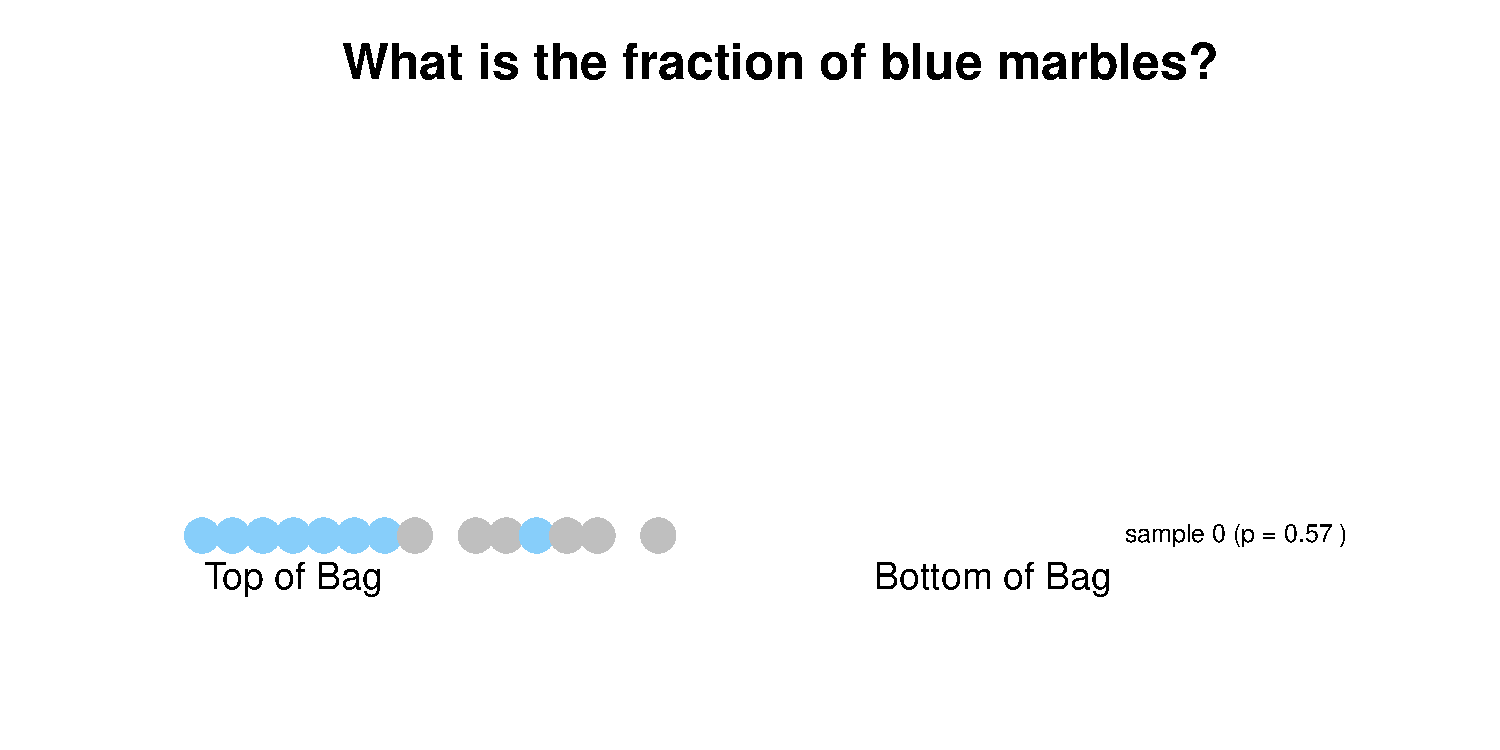
\includegraphics[scale=0.57]{bias_sample_0.pdf}
\end{center}
\end{frame}

%@@@@@@@@@@@@@@@@@@@@@@@@@@@@@@@@@@@@@@@@@@@@@@@@@
\begin{frame}
\begin{center}
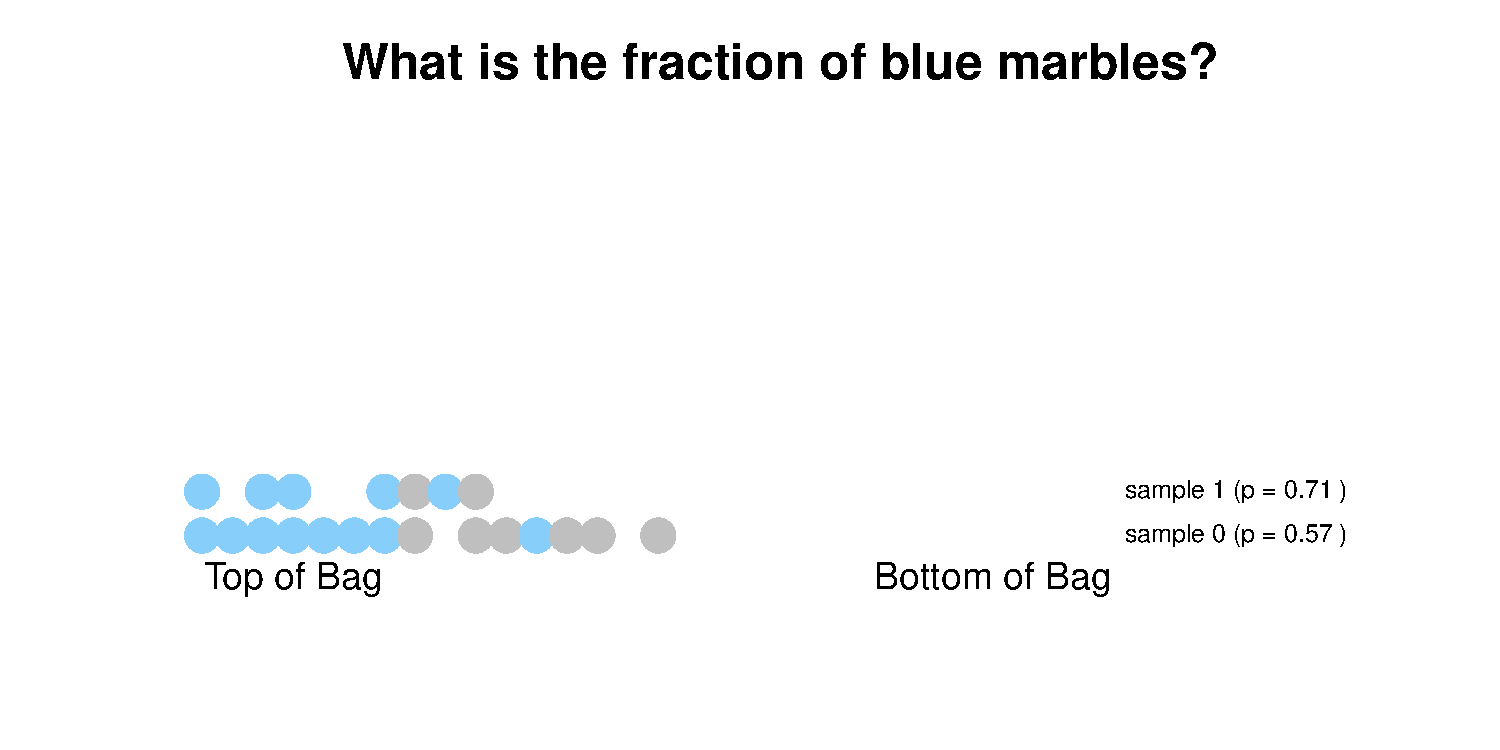
\includegraphics[scale=0.57]{bias_sample_1.pdf}
\end{center}
\end{frame}

%@@@@@@@@@@@@@@@@@@@@@@@@@@@@@@@@@@@@@@@@@@@@@@@@@
\begin{frame}
\begin{center}
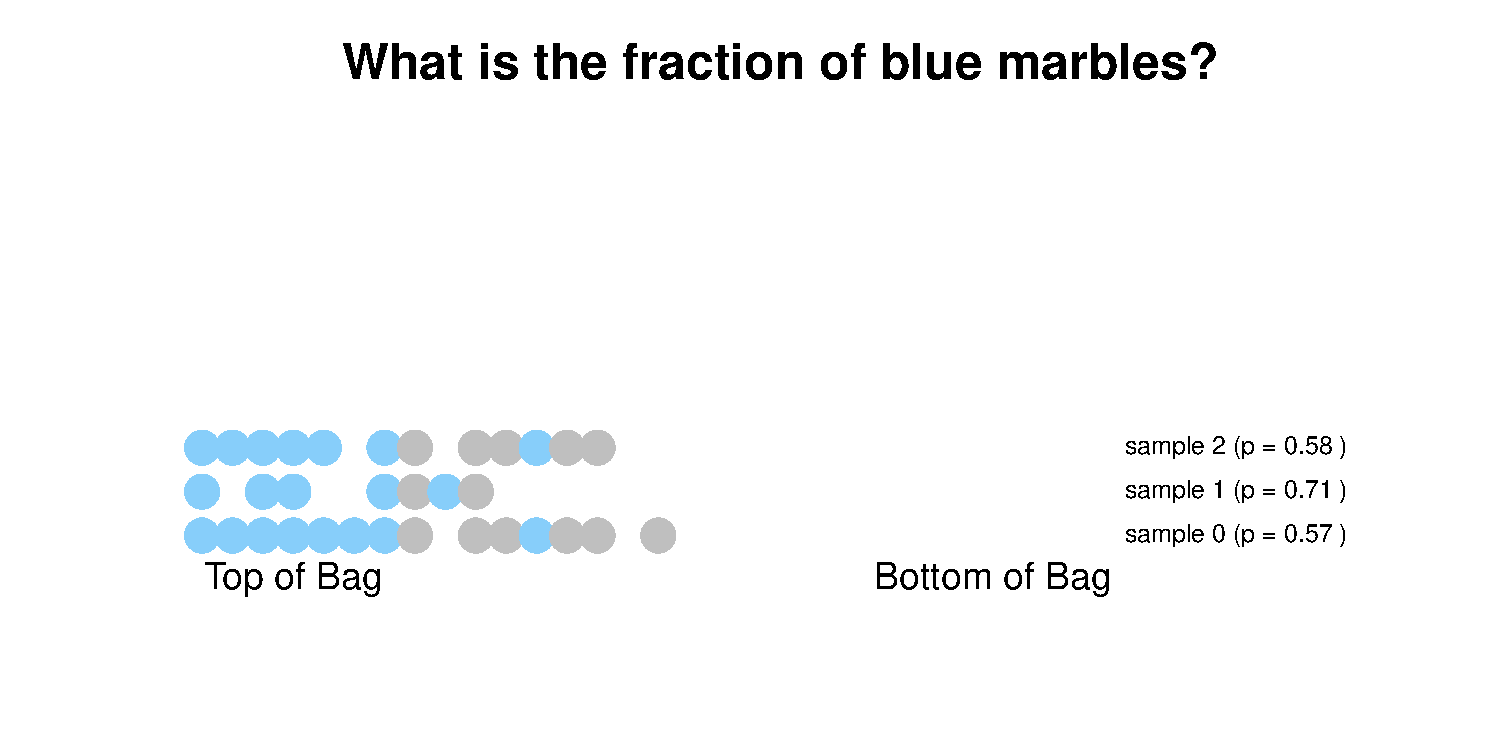
\includegraphics[scale=0.57]{bias_sample_2.pdf}
\end{center}
\end{frame}

%@@@@@@@@@@@@@@@@@@@@@@@@@@@@@@@@@@@@@@@@@@@@@@@@@
\begin{frame}
\begin{center}
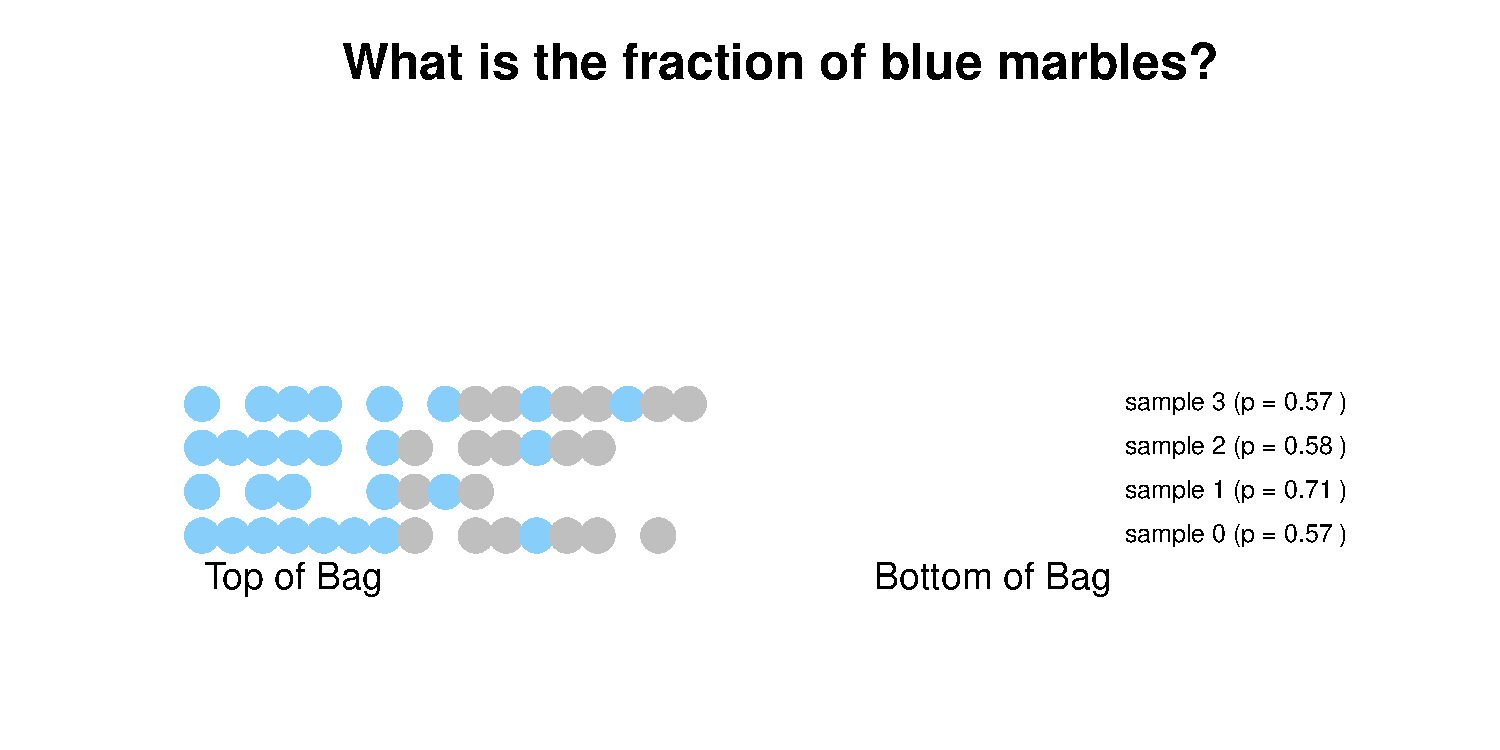
\includegraphics[scale=0.57]{bias_sample_3.pdf}
\end{center}
\end{frame}

%@@@@@@@@@@@@@@@@@@@@@@@@@@@@@@@@@@@@@@@@@@@@@@@@@
\begin{frame}
\begin{center}
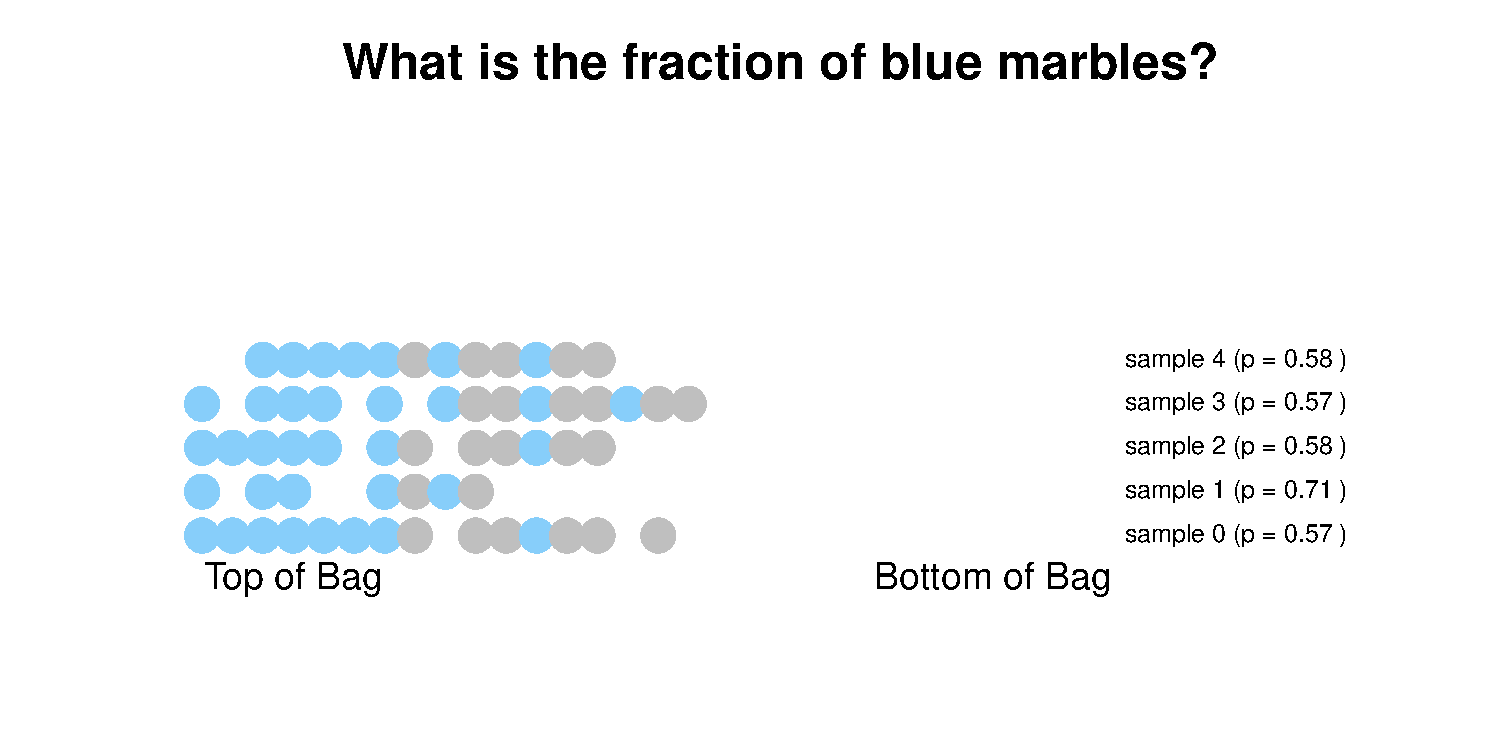
\includegraphics[scale=0.57]{bias_sample_4.pdf}
\end{center}
\end{frame}

%@@@@@@@@@@@@@@@@@@@@@@@@@@@@@@@@@@@@@@@@@@@@@@@@@
\begin{frame}
\begin{center}
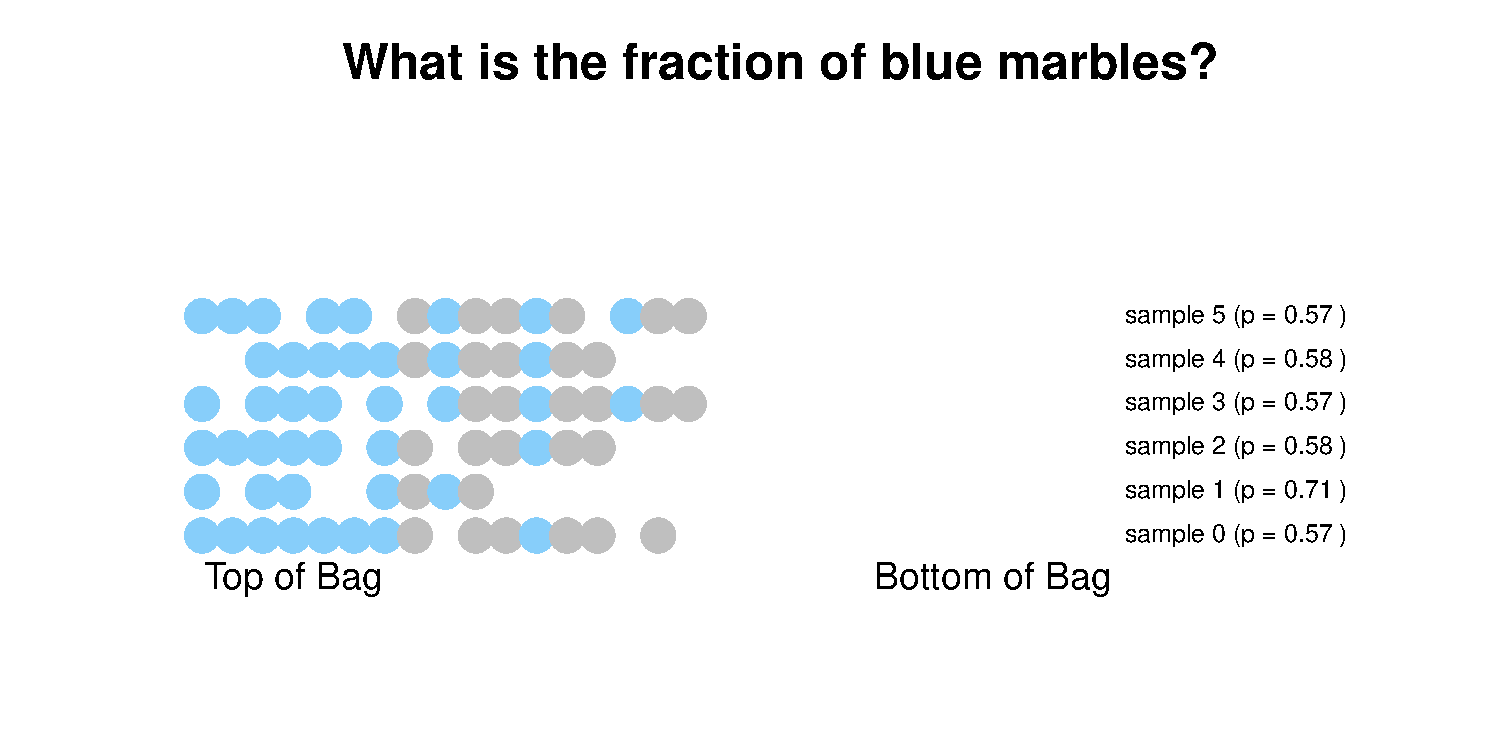
\includegraphics[scale=0.57]{bias_sample_5.pdf}
\end{center}
\end{frame}

%@@@@@@@@@@@@@@@@@@@@@@@@@@@@@@@@@@@@@@@@@@@@@@@@@
\begin{frame}
\begin{center}
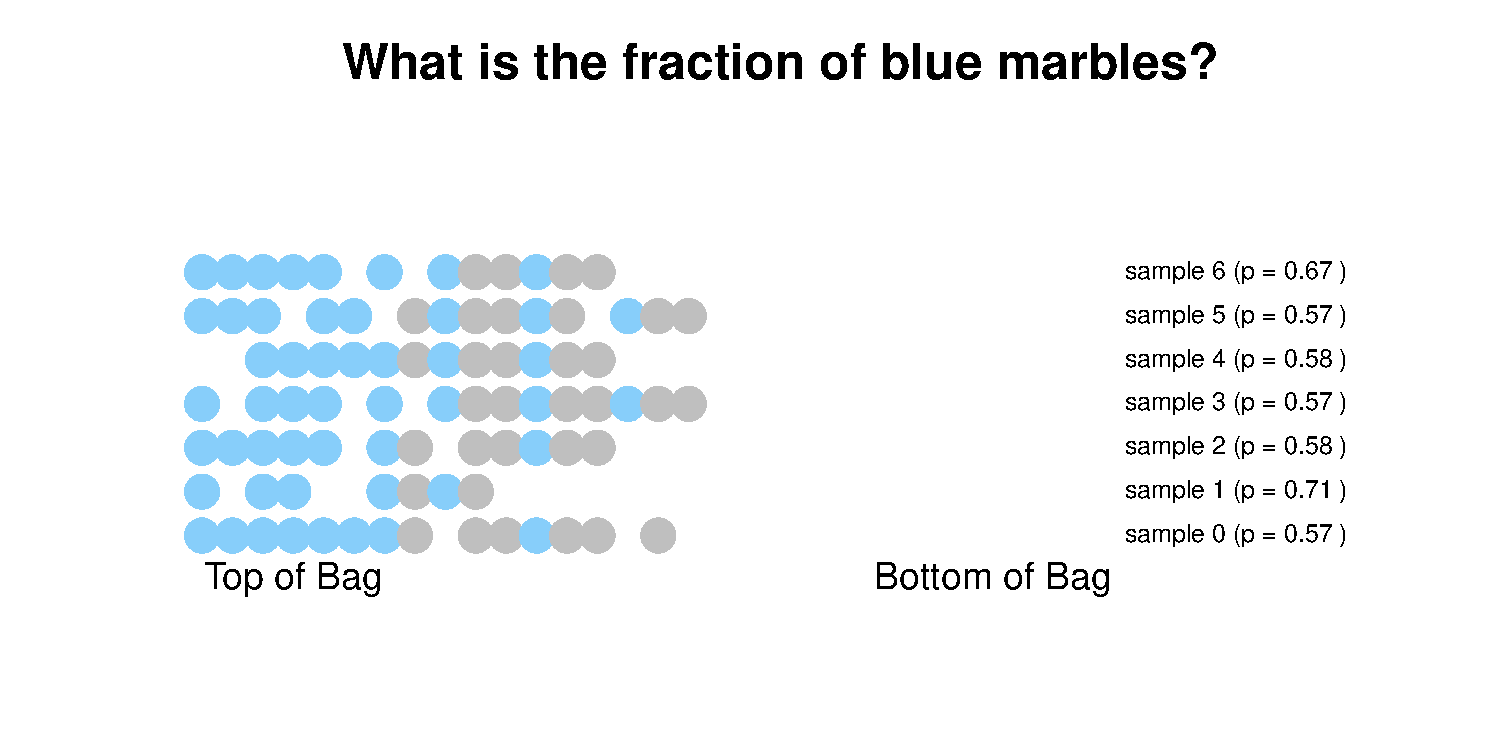
\includegraphics[scale=0.57]{bias_sample_6.pdf}
\end{center}
\end{frame}

%@@@@@@@@@@@@@@@@@@@@@@@@@@@@@@@@@@@@@@@@@@@@@@@@@
\begin{frame}
\begin{center}
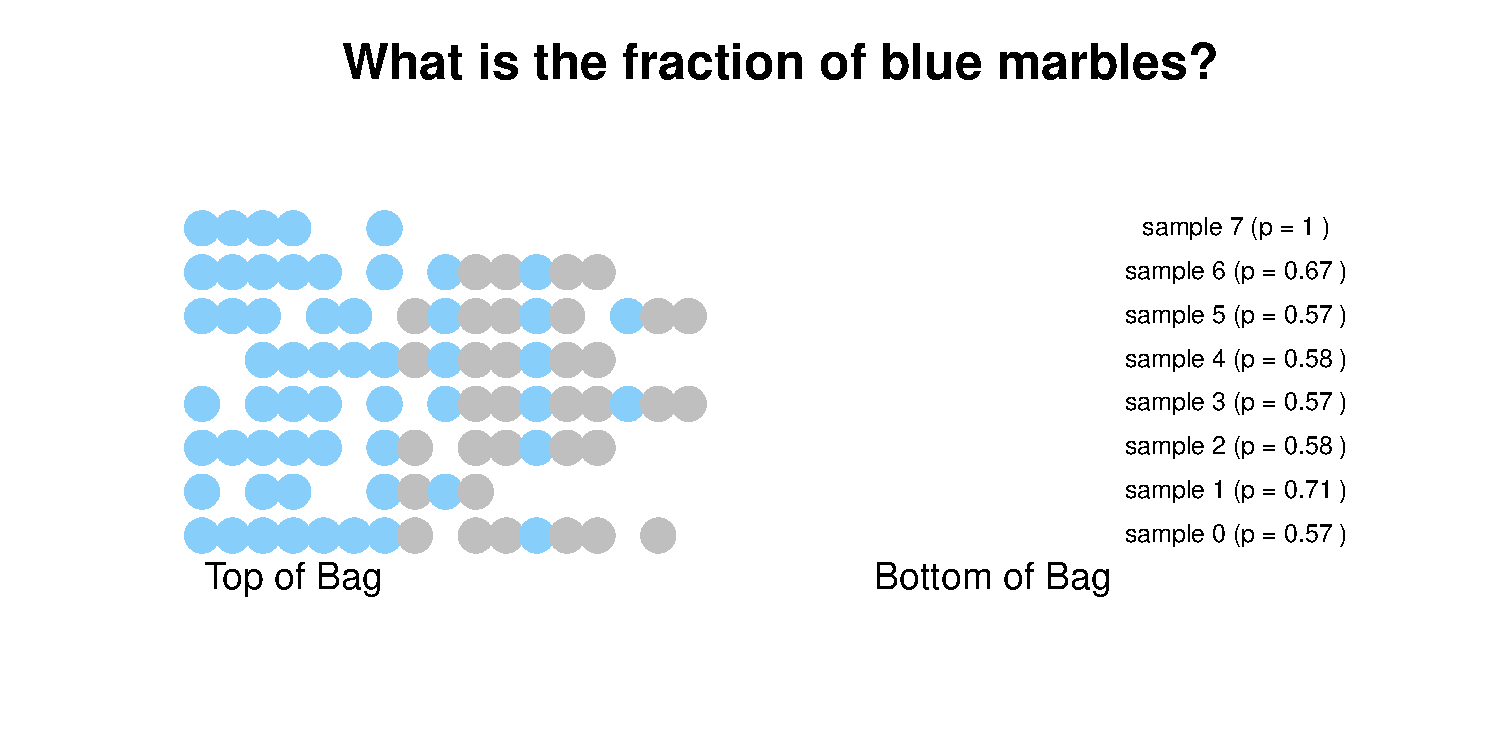
\includegraphics[scale=0.57]{bias_sample_7.pdf}
\end{center}
\end{frame}

%@@@@@@@@@@@@@@@@@@@@@@@@@@@@@@@@@@@@@@@@@@@@@@@@@
\begin{frame}
\begin{center}
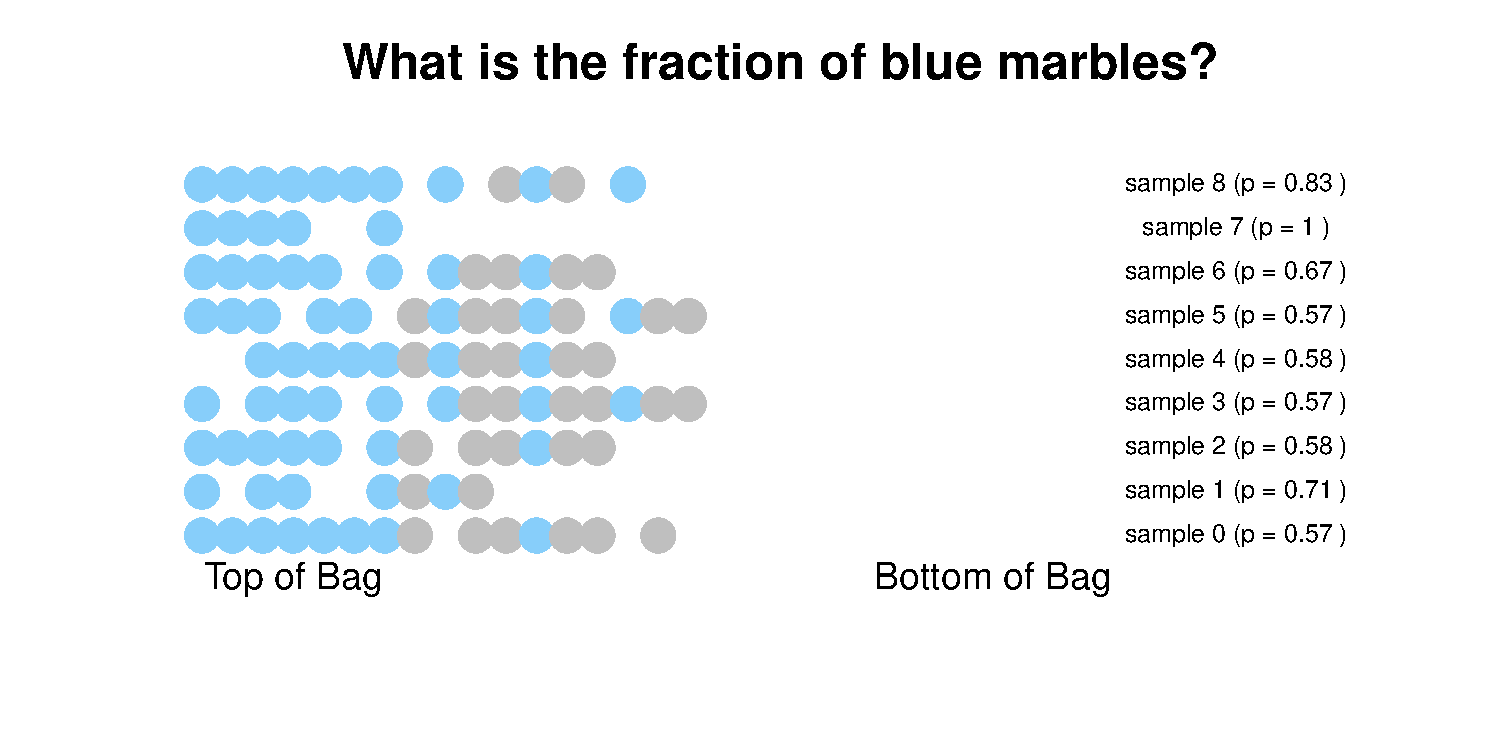
\includegraphics[scale=0.57]{bias_sample_8.pdf}
\end{center}
\end{frame}

%@@@@@@@@@@@@@@@@@@@@@@@@@@@@@@@@@@@@@@@@@@@@@@@@@
\begin{frame}
\begin{center}
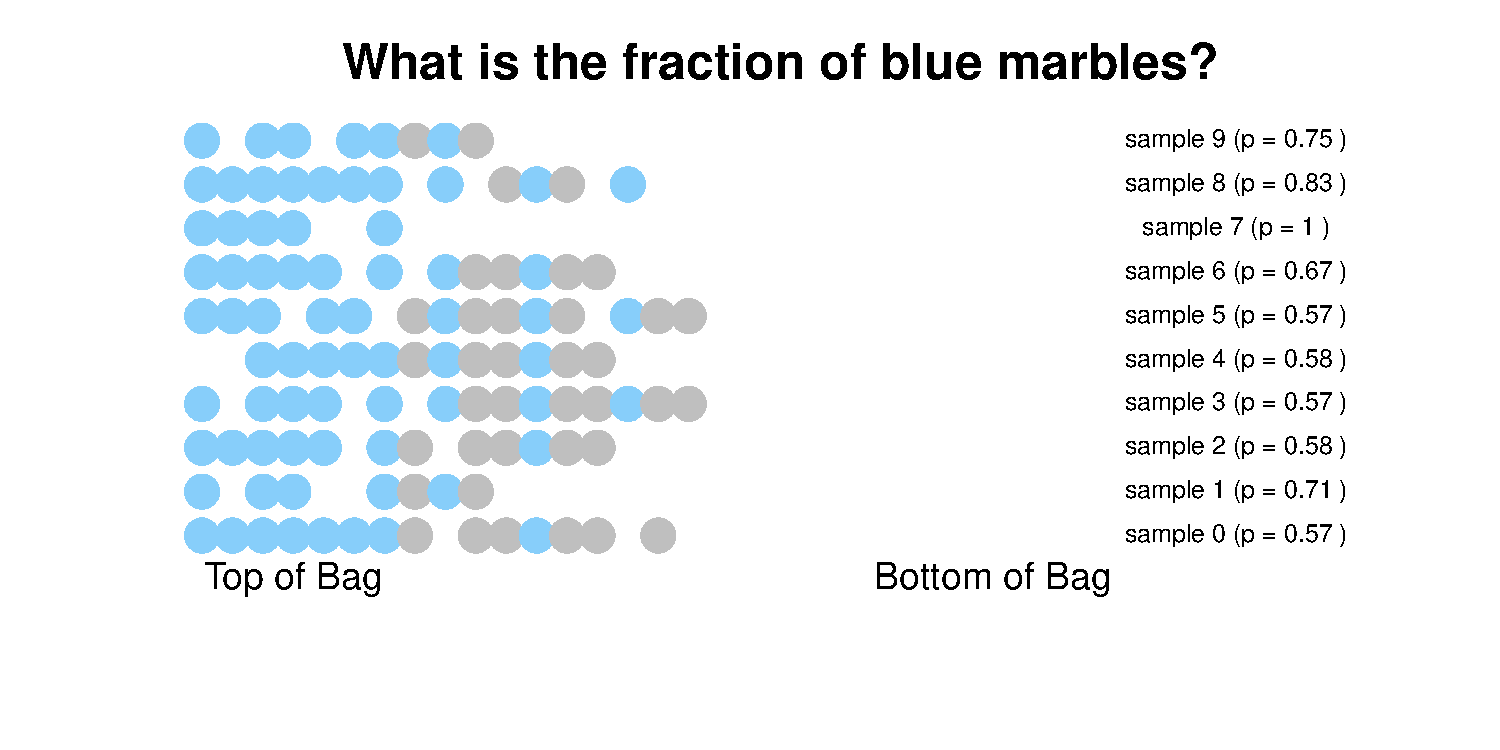
\includegraphics[scale=0.57]{bias_sample_9.pdf}
\end{center}
\end{frame}

%@@@@@@@@@@@@@@@@@@@@@@@@@@@@@@@@@@@@@@@@@@@@@@@@@
\begin{frame}
\begin{center}
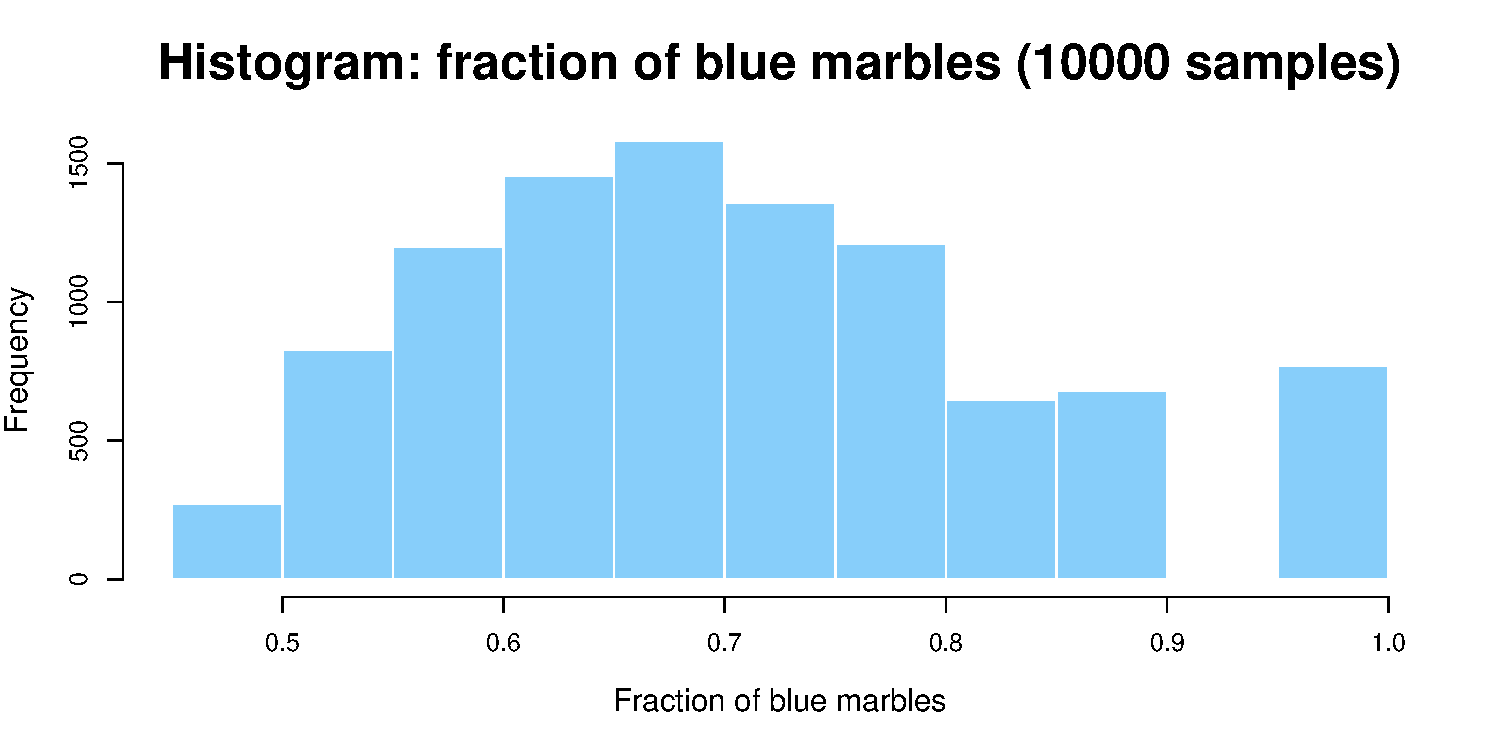
\includegraphics[scale=0.57]{bias_hist_10000_samples.pdf}
\end{center}
\end{frame}

%@@@@@@@@@@@@@@@@@@@@@@@@@@@@@@@@@@@@@@@@@@@@@@@@@
\begin{frame}
\begin{center}
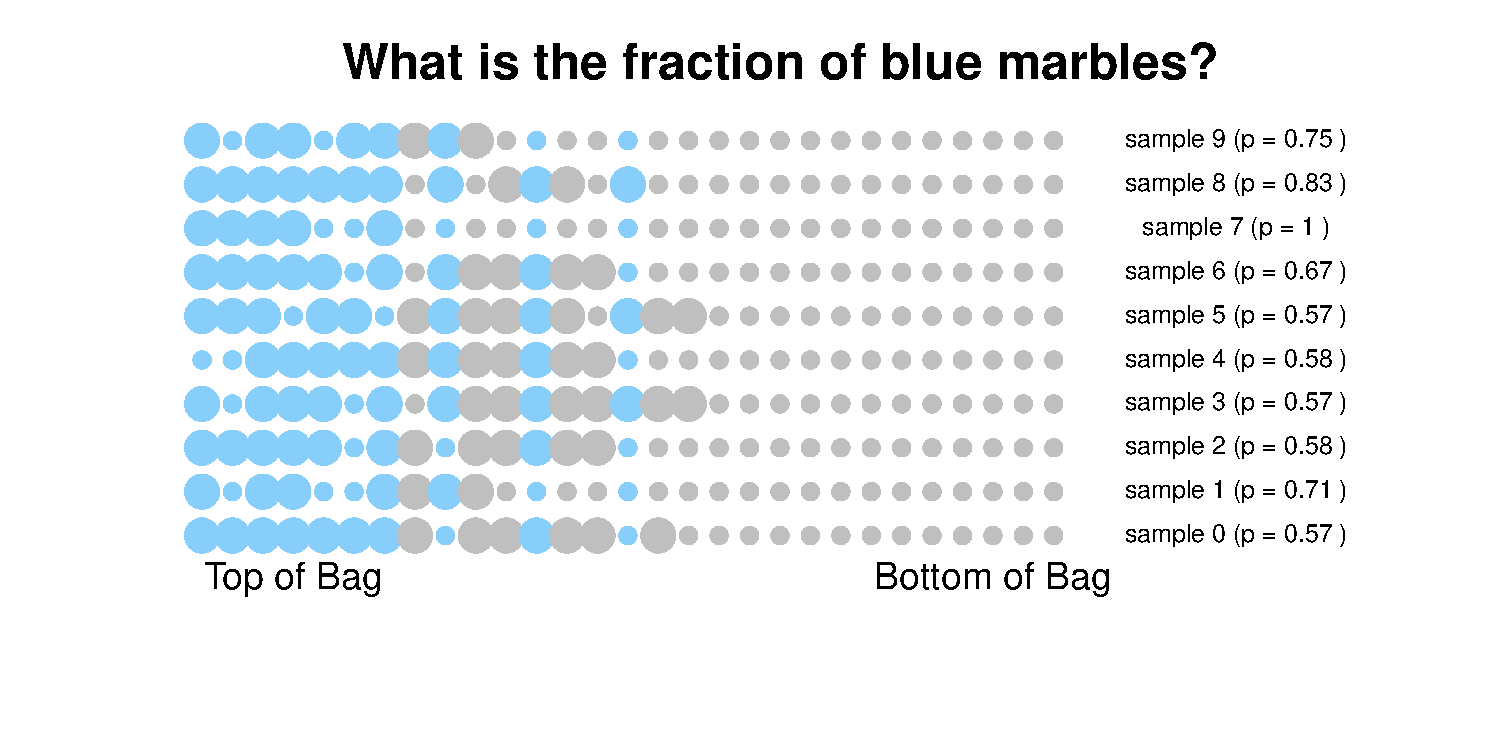
\includegraphics[scale=0.57]{bias_sample_full.pdf}
\end{center}
\end{frame}

%@@@@@@@@@@@@@@@@@@@@@@@@@@@@@@@@@@@@@@@@@@@@@@@@@
\begin{frame}
\frametitle{Sampling methodology}

\begin{itemize}
\item \textbf{Representative sample}: a sample is representative if its characteristics ``look like" the population;
\bigskip
\item \textbf{Generalizable}: a sample is generalizable if we can make ``good" guesses about the population using the characteristics of the sample;
\bigskip
\item \textbf{Bias}: a sample is biased if certain individuals in a population have a higher chance of being included in a sample than others;
\bigskip
\item[]\color{white} In general if we create a sample of size $n$ randomly then...
\begin{itemize}
\item[]\color{white} ...the sample will be unbiased and representative of the population of size $N$ so...
\item[]\color{white} ...any result based on the sample with generalize to the population and therefore...
\item[]\color{white} ...the sample statistic is a good guess for the population parameter which means...
\item[]\color{white} ...that we can \textbf{INFER} about the population using the sample.
\end{itemize}
\bigskip
\item[]\color{white} Our second experiment is an example of a \textbf{selection effect} -- selection of a biased sample that was not representative and so not generalizable.
\end{itemize}

\end{frame}

%@@@@@@@@@@@@@@@@@@@@@@@@@@@@@@@@@@@@@@@@@@@@@@@@@
\begin{frame}
\frametitle{Sampling methodology}

\begin{itemize}
\item \textbf{Representative sample}: a sample is representative if its characteristics ``look like" the population;
\bigskip
\item \textbf{Generalizable}: a sample is generalizable if we can make ``good" guesses about the population using the characteristics of the sample;
\bigskip
\item \textbf{Bias}: a sample is biased if certain individuals in a population have a higher chance of being included in a sample than others;
\bigskip
\item In general if we create a sample of size $n$ randomly then...
\begin{itemize}
\item ...the sample will be unbiased and representative of the population of size $N$ so...
\item ...any result based on the sample with generalize to the population and therefore...
\item ...the sample statistic is a good guess for the population parameter which means...
\item ...that we can \textbf{INFER} about the population using the sample.
\end{itemize}
\bigskip
\item Our second experiment is an example of a \textbf{selection effect} -- selection of a biased sample that was not representative and so not generalizable.
\end{itemize}

\end{frame}

%@@@@@@@@@@@@@@@@@@@@@@@@@@@@@@@@@@@@@@@@@@@@@@@@@
\begin{frame}
\frametitle{An IRL example: polling in 1936...}

\begin{columns}
\begin{column}{0.5\textwidth}

\begin{itemize}
\item \textit{The Literary Digest}:
\begin{itemize}
\item A weekly magazine that started in 1890 w/ circulation $> 1,000,000$;
\item Correctly predicted US presidential elections from 1916 -- 1932;
\end{itemize}

\item 1936 Election: Langdon v Roosevelt;
\begin{itemize}
\item \textit{The Literary Digest} polled 10 million and got 2.3 million responses;
\item Langdon predicted to be the decisive winner -- but Roosevelt crushed him!
\end{itemize}

\item The magazine folded within 18 months -- what happened?! \color{white} Sampled:
\begin{itemize}
\item[]\color{white} Auto registrations;
\item[]\color{white} Phone number lists;
\item[]\color{white} Country club memberships;
\item[]\color{white} Its own subscriber list.
\end{itemize}
\end{itemize}

\end{column}
\begin{column}{0.5\textwidth}
\begin{center}
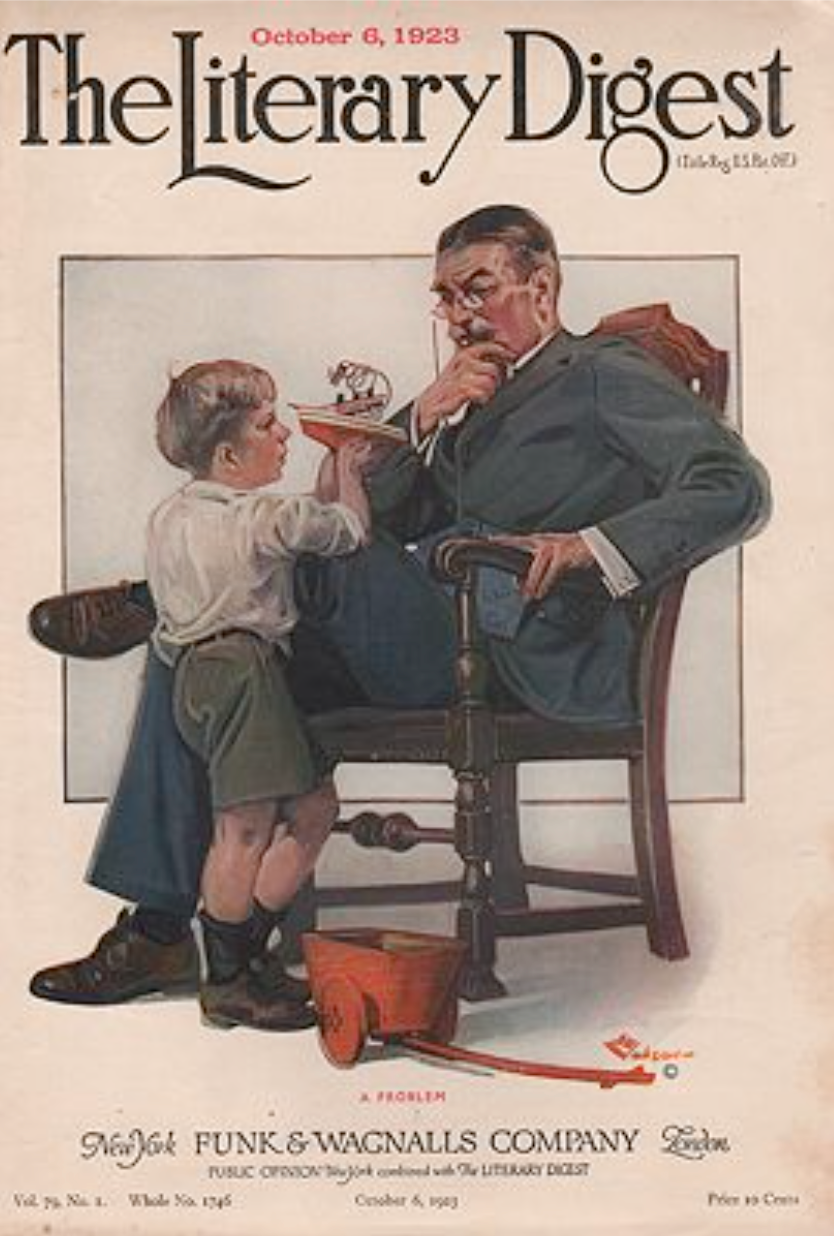
\includegraphics[scale=0.3]{LD.png}
\end{center}
\end{column}
\end{columns}

\end{frame}

%@@@@@@@@@@@@@@@@@@@@@@@@@@@@@@@@@@@@@@@@@@@@@@@@@
\begin{frame}
\frametitle{An IRL example: polling in 1936...}

\begin{columns}
\begin{column}{0.5\textwidth}

\begin{itemize}
\item \textit{The Literary Digest}:
\begin{itemize}
\item A weekly magazine that started in 1890 w/ circulation $> 1,000,000$;
\item Correctly predicted US presidential elections from 1916 -- 1932;
\end{itemize}

\item 1936 Election: Langdon v Roosevelt;
\begin{itemize}
\item \textit{The Literary Digest} polled 10 million and got 2.3 million responses;
\item Langdon predicted to be the decisive winner -- but Roosevelt crushed him!
\end{itemize}

\item The magazine folded within 18 months -- what happened?!  Sampled:
\begin{itemize}
\item Auto registrations;
\item Phone number lists;
\item Country club memberships;
\item Its own subscriber list.
\end{itemize}
\end{itemize}

\end{column}
\begin{column}{0.5\textwidth}
\begin{center}
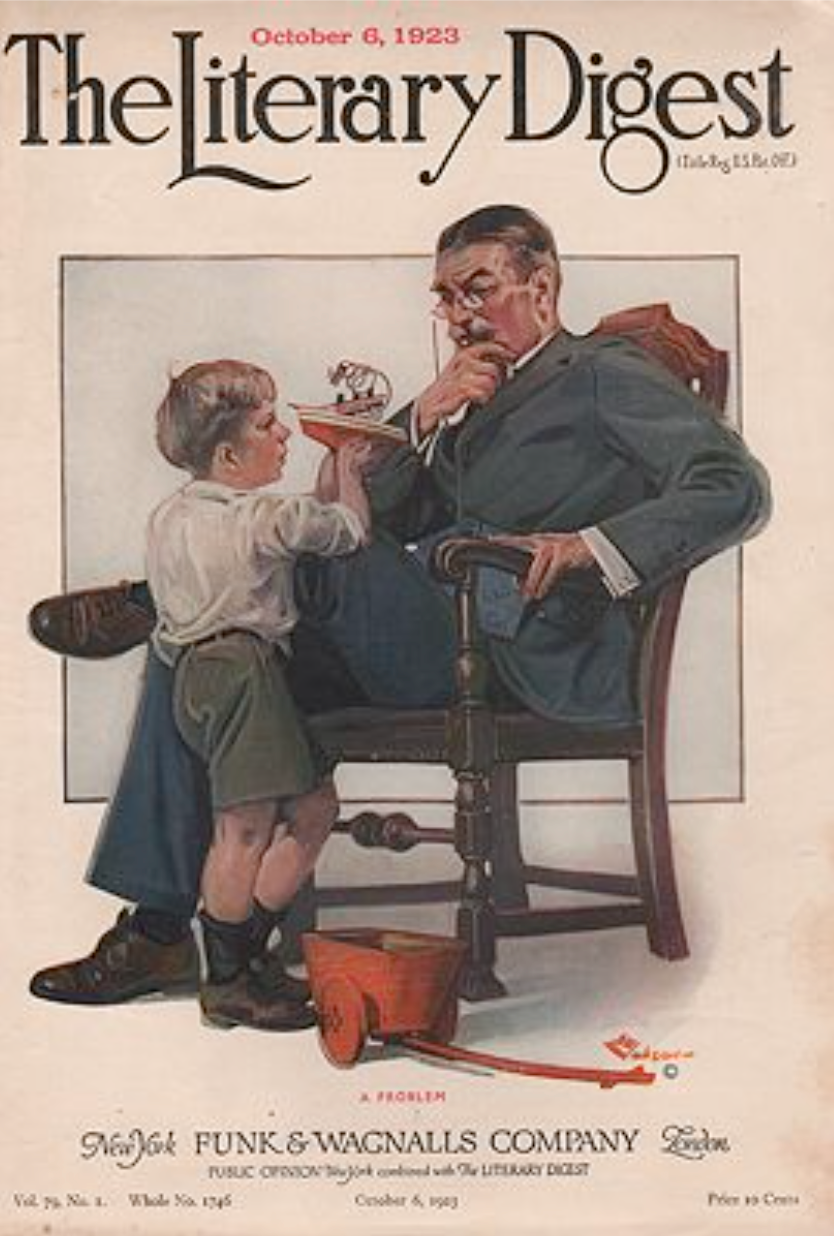
\includegraphics[scale=0.3]{LD.png}
\end{center}
\end{column}
\end{columns}

\end{frame}

%@@@@@@@@@@@@@@@@@@@@@@@@@@@@@@@@@@@@@@@@@@@@@@@@@
\begin{frame}
\frametitle{What happens as we take more samples?}

\begin{itemize}
\item So why is it that the most frequent value in the histogram appeared to get closer and closer to the actual value of $\frac{1}{3}$ as we added samples?
\bigskip
\bigskip
\bigskip
\item \textbf{Theorem} (Weak Law of Large Numbers, informal): the sample average ``moves towards" the ``true" value as the number of samples grows.

\end{itemize}

\end{frame}

%%@@@@@@@@@@@@@@@@@@@@@@@@@@@@@@@@@@@@@@@@@@@@@@@@@
%\begin{frame}
%\frametitle{What happens as we take more samples?}
%
%\begin{itemize}
%\item So why is it that the most frequent value in the histogram appeared to get closer and closer to the actual value of $\frac{1}{3}$ as we added samples?
%\bigskip
%\bigskip
%\item \textbf{Theorem} (Weak Law of Large Numbers, informal): the sample average ``moves towards" the ``true" value as the number of samples grows.
%\bigskip
%\bigskip
%\item \textbf{Theorem} (Weak Law of Large Numbers, formal): Given samples $X_1, X_2, \hdots, X_n$ for any $\varepsilon>0$:
%\begin{align*}
%\lim_{n\to\infty}\mbox{Probability}\left(\left|\frac{1}{n}\sum_{i=1}^nX_i - \mu\right| < \varepsilon\right) = 1.
%\end{align*}
%\end{itemize}
%
%\end{frame}

\begin{frame}
\frametitle{What happens as sample size grows?}

\begin{itemize}
\item Why is it that the sampling distribution got more peaked as we increased the sample size?
\bigskip
\bigskip
\bigskip
\item \textbf{Theorem} (Central Limit Theorem): As sample size gets bigger the sampling distribution of a sample statistic increasingly follows a normal distribution and the standard deviation of that normal distribution gets smaller.
%\bigskip
%\bigskip
%\item \textbf{Theorem} (Central Limit Theorem, formal): Blar.
\end{itemize}

\end{frame}

%@@@@@@@@@@@@@@@@@@@@@@@@@@@@@@@@@@@@@@@@@@@@@@@@@
\begin{frame}
\frametitle{Data Generating Process}

\begin{itemize}
\item A useful (and ubiquitous) construct: \textbf{the data generating process} (DGP) -- the set of all operations that lead to:
\begin{enumerate}
\item the particular observations that appear in the dataset...
\item ...and their structure;
\end{enumerate}
\bigskip
\item Occurs both IRL and at the researcher's desk -- usually we know at most only part of the DGP;
\bigskip
\item Selected examples:
\begin{enumerate}
\item Generation of events (could become data) -- e.g. some countries fight wars;
\item Selection of population units into the data;
\item Categorization/Binarization -- e.g. a Likert scale representation of preference;
\item Analyst decisions to aggregate, group, or drop data;
\item Assignment of independent variables to observations (e.g. selection of treatment and control groups);
\end{enumerate}
\bigskip
\item[] \color{white}Depending on who controls (4) the data can be either experimental or observational.
\end{itemize}

\end{frame}

%@@@@@@@@@@@@@@@@@@@@@@@@@@@@@@@@@@@@@@@@@@@@@@@@@
\begin{frame}
\frametitle{Data Generating Process: Sampling}

\begin{itemize}
\item A useful (and ubiquitous) construct: \textbf{the data generating process} (DGP) -- the set of all operations that lead to:
\begin{enumerate}
\item the particular observations that appear in the dataset...
\item[]\color{gray} ...and their structure;
\end{enumerate}
\bigskip
\item[]\color{gray} Occurs both IRL and at the researcher's desk -- usually we know at most only part of the DGP;
\bigskip
\item Selected examples:
\begin{enumerate}
\item \textbf{Generation of events (could become data) -- e.g. some countries fight wars};
\item \textbf{Selection of selection of population units into the data};
\item[]\color{gray} Categorization/Binarization -- e.g. a Likert scale representation of preference;
\item[]\color{gray} Analyst decisions to aggregate, group, or drop data;
\item[]\color{gray} Assignment of independent variables to observations (e.g. selection of treatment and control groups);
\end{enumerate}
\bigskip
\item[] \color{white}Depending on who controls (4) the data can be either experimental or observational.
\end{itemize}

\end{frame}

%@@@@@@@@@@@@@@@@@@@@@@@@@@@@@@@@@@@@@@@@@@@@@@@@@
\begin{frame}

\begin{center}
\Huge\textbf{Why should we care?}\\
\bigskip
\bigskip
\large Concepts of sampling will be the basis of things like probability and hypothesis testing which we will cover next!  Understanding sampling methodology will help you decide whether to trust polling results etc.\\
\end{center}

\end{frame}



\end{document}






